%=========================================================
\chapter{Modelo dinámico}	
\label{cap:modDinamico}

	Este capítulo describe en modelo dinámico del sistema. en el se detallan todos los escenarios de ejecución del sistema. La figura~\ref{fig:casosDeUso} muestra el diagrama general del sistema y sus sib sistemas, y la figura~\ref{fig:casosDeUsoDetalle} muestra todos los casos de uso del sistema. En este documento solo detallamos los casos de uso del subsistema de gestión de cursos.
	
\begin{figure}[htbp]
	\begin{center}
		\fbox{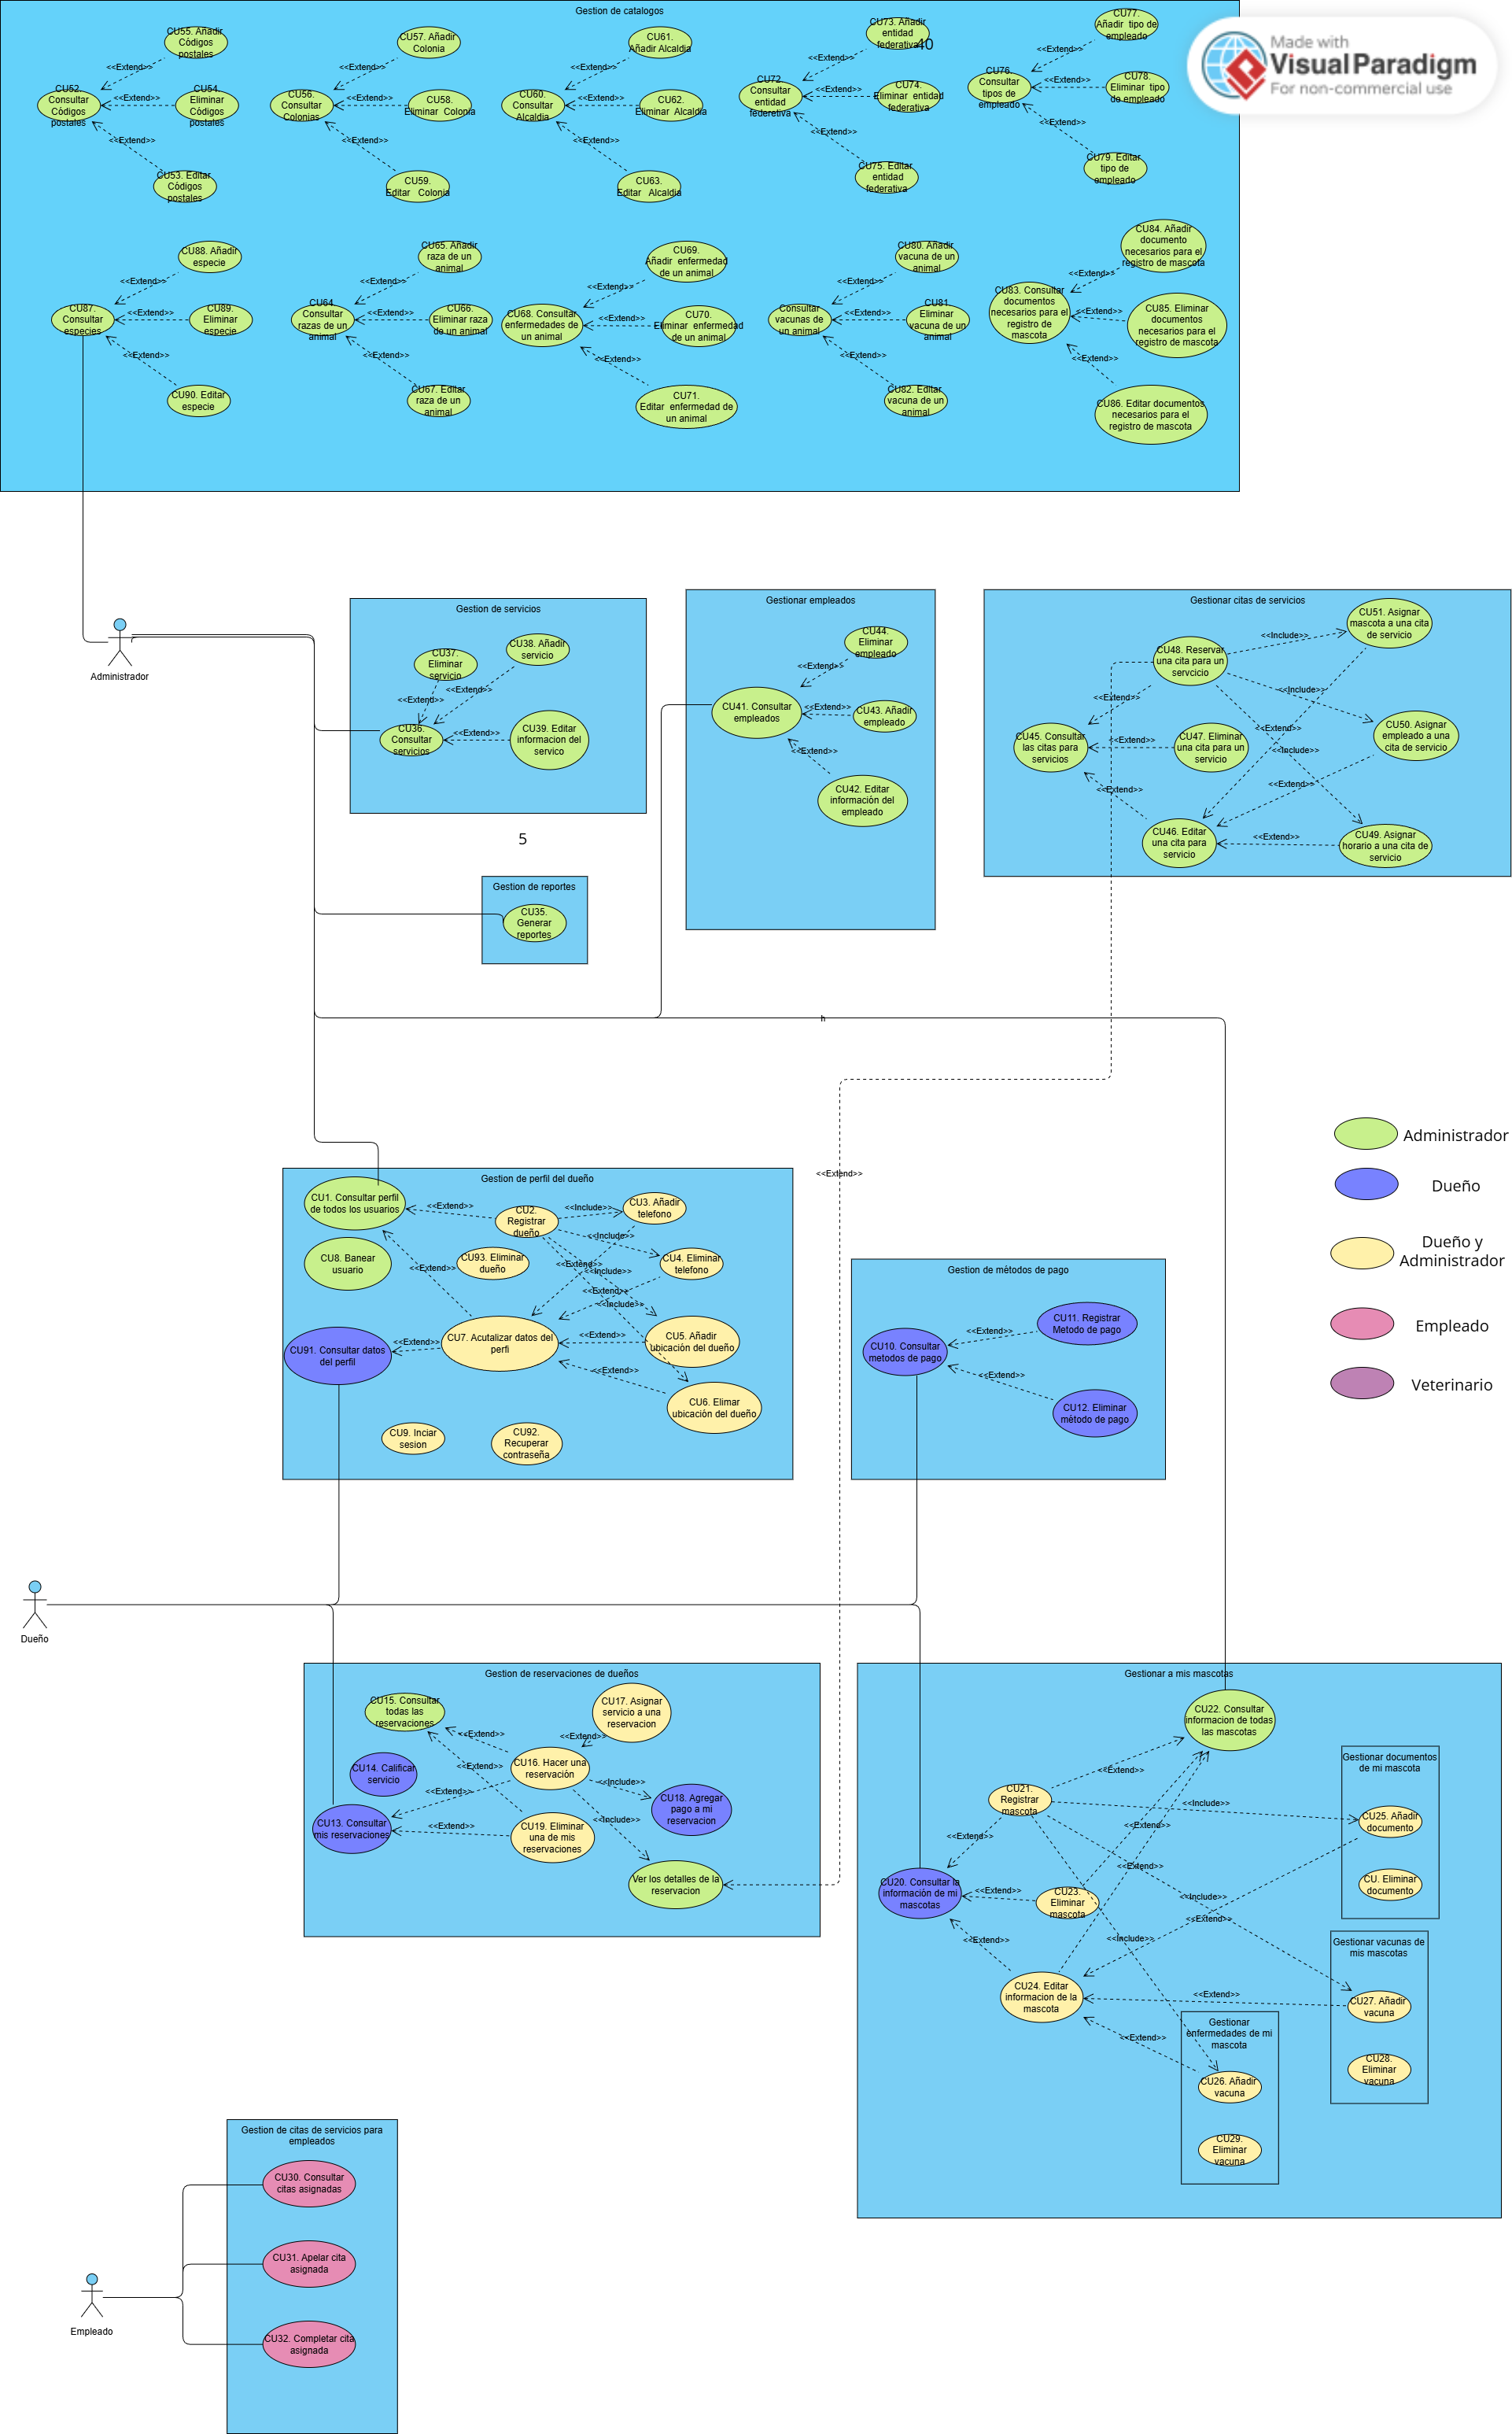
\includegraphics[width=.8\textwidth]{images/casosDeUso}}
		\caption{Diagrama de casos de uso del sistema.}
		\label{fig:casosDeUso}
	\end{center}
\end{figure}

\begin{figure}[htbp]
	\begin{center}
		\includegraphics[angle=90, width=.7\textwidth]{images/casosDeUsoDetalle}
		\caption{Diagrama detallado del sistema.}
		\label{fig:casosDeUsoDetalle}
	\end{center}
\end{figure}

%---------------------------------------------------------
\section{Descripción de actores}

%---------------------------------------------------------
\begin{Usuario}{\hypertarget{Propietario}{\subsection{Propietario}}}{
	Es el dueño de una o más mascotas que utiliza el sistema para gestionar la información de sus animales y realizar reservaciones de servicios del hotel canino.
}
    \item[Responsabilidades:] \cdtEmpty
    \begin{itemize}
		\item Registrar y mantener actualizada la información de sus mascotas (datos personales, historial médico, vacunas, alergias, documentos).
		\item Crear, consultar, modificar y cancelar reservaciones para hospedaje de sus mascotas.
		\item Gestionar sus datos personales (información de contacto, direcciones, teléfonos).
		\item Realizar pagos por los servicios contratados.
		\item Consultar el historial de servicios y reservaciones de sus mascotas.
    \end{itemize}

	\item[Perfil:] \cdtEmpty
    \begin{itemize}
		\item Dueño de una o más mascotas.
		\item Usuario registrado en el sistema con correo electrónico y contraseña.
		\item Rol asignado: Cliente (rol\_id = 2).
		\item Conocimientos básicos de navegación web o uso de aplicaciones móviles.
    \end{itemize}
\end{Usuario}

%---------------------------------------------------------
\begin{Usuario}{\hypertarget{Administrador}{\subsection{Administrador}}}{
	Es el personal del hotel canino con privilegios administrativos para gestionar el sistema, los empleados, servicios y habitaciones.
}
    \item[Responsabilidades:] \cdtEmpty
    \begin{itemize}
		\item Gestionar catálogos del sistema (especies, razas, enfermedades, servicios, habitaciones).
		\item Administrar información de empleados y asignar especialidades.
		\item Supervisar y gestionar reservaciones de todos los clientes.
		\item Asignar habitaciones y servicios a las reservaciones.
		\item Configurar citas de servicios y asignar empleados responsables.
		\item Generar reportes y consultas del sistema.
		\item Mantener la integridad y seguridad de la información.
    \end{itemize}

	\item[Perfil:] \cdtEmpty
    \begin{itemize}
		\item Empleado del hotel canino con rol administrativo.
		\item Usuario registrado con rol: Admin (rol\_id = 1).
		\item Conocimiento completo del funcionamiento del hotel y sus procesos.
		\item Capacidad para tomar decisiones sobre asignación de recursos.
		\item Experiencia en sistemas de gestión y atención al cliente.
    \end{itemize}
\end{Usuario}

%---------------------------------------------------------
\begin{Usuario}{\hypertarget{Empleado}{\subsection{Empleado}}}{
	Es el personal operativo del hotel que brinda servicios directos a las mascotas (veterinarios, peluqueros, cuidadores, etc.).
}
    \item[Responsabilidades:] \cdtEmpty
    \begin{itemize}
		\item Ejecutar los servicios asignados en las citas programadas.
		\item Brindar atención veterinaria, peluquería, entrenamiento u otros servicios especializados.
		\item Registrar notas y observaciones sobre los servicios brindados.
		\item Consultar información relevante de las mascotas bajo su cuidado (alergias, enfermedades, historial).
		\item Reportar incidencias o situaciones especiales al administrador.
    \end{itemize}

	\item[Perfil:] \cdtEmpty
    \begin{itemize}
		\item Personal capacitado en el cuidado y atención de mascotas.
		\item Especialidad definida: veterinaria, peluquería, entrenamiento, cuidado general.
		\item Certificaciones o licencias profesionales según la especialidad (ej. médico veterinario).
		\item Experiencia práctica en el trato con animales.
		\item Capacidad para seguir protocolos de seguridad e higiene.
    \end{itemize}
\end{Usuario}

A continuación se detallan los casos de uso.

%---------------------------------------------------------
% CASOS DE USO

%-------------------------------------- COMIENZA descripción del caso de uso.

  \begin{UseCase}{CU01}{Crear Mascota}{
      Permite al Propietario registrar una nueva mascota en el sistema, asociándola a su perfil para la gestión de su información y futuras reservaciones.
  }
      \UCitem{Versión}{\color{Gray}1.0}
      \UCitem{Autor}{\color{Gray}Castillo Aldaba Jared}
      \UCitem{Supervisa}{\color{Gray}Ugalde Tellez Aaron}
      \UCitem{Actor}{\hyperlink{Propietario}{Propietario}}
      \UCitem{Propósito}{Registrar los datos de una nueva mascota para gestionar su perfil, historial médico y futuras reservaciones.}
      \UCitem{Entradas}{
          \begin{itemize}
              \item \textbf{nombre}
              \item \textbf{especie\_id}
              \item \textbf{sexo\_id}
              \item \textbf{fecha\_nacimiento}
              \item Datos opcionales: raza\_id, peso\_kg, esterilizado, señas particulares, etc.
          \end{itemize}
      }
      \UCitem{Origen}{Teclado / Mouse}
      \UCitem{Salidas}{Mensaje de confirmación, Lista de mascotas actualizada.}
      \UCitem{Destino}{Pantalla y Base de Datos}
      \UCitem{Precondiciones}{
          \begin{itemize}
              \item El Propietario debe haber iniciado sesión en el sistema.
              \item El Propietario se encuentra en la pantalla de gestión de sus mascotas.
          \end{itemize}
      }
      \UCitem{Postcondiciones}{Se crea un nuevo registro en la tabla mascotas con los datos proporcionados, asociado al propietario\_id del usuario autenticado.}
      \UCitem{Errores}{
          \begin{itemize}
              \item \textbf{E1}: Datos de formulario inválidos o incompletos.
              \item \textbf{E2}: Usuario no autenticado o sesión expirada.
              \item \textbf{E3}: Error de conexión con el servidor.
          \end{itemize}
      }
      \UCitem{Tipo}{Primario}
  \end{UseCase}

  %--------------------------------------
  % Trayectoria Principal
  %--------------------------------------
  \begin{UCtrayectoria}
      \UCpaso[\UCactor] Accede a la \IUref{IU-PetList}{Lista de Mascotas} y oprime el botón \IUbutton{Agregar Mascota}.
      \UCpaso Despliega la \IUref{IU-PetForm}{Formulario de Mascota}.
      \UCpaso[\UCactor] Introduce los datos de la mascota en los campos correspondientes. \label{CU-CreatePet-FillForm}
      \UCpaso[\UCactor] Oprime el botón \IUbutton{Crear Mascota}.
      \UCpaso Verifica que los datos obligatorios (nombre, especie, sexo, fecha de nacimiento) estén completos y tengan el formato correcto con base en la regla \BRref{BR-PetValidation}{Validación de Datos de Mascota}.
      \UCpaso Solicita al servidor la creación del registro.
      \UCpaso El sistema verifica que el usuario esté autenticado y tenga permisos.
      \UCpaso El sistema registra la nueva mascota en la base de datos.
      \UCpaso Muestra el mensaje de éxito {\bf MSG1-}``Mascota creada exitosamente''.
      \UCpaso Actualiza la \IUref{IU-PetList}{Lista de Mascotas} para mostrar la nueva mascota.
  \end{UCtrayectoria}
  
  %--------------------------------------
  % Trayectorias Alternativas
  %--------------------------------------
  
  % Trayectoria A: Datos Inválidos
  \begin{UCtrayectoriaA}{A}{El Propietario ingresa datos inválidos}
      \UCpaso El sistema detecta que uno o más campos obligatorios están vacíos o tienen un formato incorrecto.
      \UCpaso Muestra el mensaje de error {\bf MSG-Error} ``Por favor completa todos los campos requeridos''.
      \UCpaso Resalta los campos con errores en el formulario.
      \UCpaso[\UCactor] Oprime el botón \IUbutton{Aceptar}.
      \UCpaso Continúa en el paso 5 de la trayectoria principal.
  \end{UCtrayectoriaA}
  
  % Trayectoria B: Sesión Expirada
  \begin{UCtrayectoriaA}{B}{La sesión del Propietario ha expirado}
      \UCpaso El sistema detecta que el token de autenticación es inválido o ha expirado.
      \UCpaso Muestra el mensaje de error {\bf MSG-Error} ``Tu sesión ha expirado. Por favor, inicia sesión de nuevo.''.
      \UCpaso Redirige al usuario a la \IUref{IU-Login}{Pantalla de Inicio de Sesión}.
      \UCpaso Termina el caso de uso.
  \end{UCtrayectoriaA}
  
  % Trayectoria C: Fallo del Sistema
  \begin{UCtrayectoriaA}{C}{Fallo inesperado del sistema}
      \UCpaso Ocurre un error interno en el servidor al intentar registrar la mascota.
      \UCpaso Muestra el mensaje de error {\bf MSG-Error} ``Ocurrió un error al procesar tu solicitud. Por favor, intenta más tarde.''.
      \UCpaso[\UCactor] Oprime el botón \IUbutton{Aceptar}.
      \UCpaso[] El sistema permanece en el \IUref{IU-PetForm}{Formulario de Mascota}, permitiendo al usuario reintentar la operación.
  \end{UCtrayectoriaA}
%--------------------------------------
% Puntos de extensión
%--------------------------------------
\subsection{Puntos de extensión}
\UCExtenssionPoint{
	% Cuando:
	El propietario desea ver el perfil completo y agregar más detalles (vacunas, enfermedades, etc.) a la mascota recién creada.
}{
	% Durante la región:
	Paso 10 (Visualización de la lista actualizada).
}{
	% Casos de uso a los que extiende:
	\hyperlink{CU14}{CU14 Consultar Detalle de Mascota}, \hyperlink{CU06}{CU06 Agregar Historial Médico}.
}

\UCExtenssionPoint{
	% Cuando:
	El propietario desea crear una reservación para la mascota recién creada.
}{
	% Durante la región:
	Paso 10 (Visualización de la lista actualizada).
}{
	% Casos de uso a los que extiende:
	\hyperlink{CU15}{CU15 Crear Reservación}.
}

%-------------------------------------- TERMINA descripción del caso de uso.


%-------------------------------------- COMIENZA descripción del caso de uso.

\begin{UseCase}{CU02}{Eliminar Mascota}{
	Permite al Propietario eliminar de forma permanente el registro de una de sus mascotas del sistema, por ejemplo, en caso de un registro erróneo o duplicado.
}
	\UCitem{Versión}{\color{Gray}1.0}
	\UCitem{Autor}{\color{Gray}Analista de Sistemas}
	\UCitem{Supervisa}{\color{Gray}[Nombre del Supervisor]}
	\UCitem{Actor}{\hyperlink{Propietario}{Propietario}}
	\UCitem{Propósito}{Mantener actualizada la lista de mascotas activas del propietario, eliminando registros que ya no son necesarios.}
	\UCitem{Entradas}{
		\begin{itemize}
			\item Selección de la mascota a eliminar desde la lista.
			\item Confirmación de la acción de borrado.
		\end{itemize}
	}
	\UCitem{Origen}{Mouse / Pantalla táctil}
	\UCitem{Salidas}{Mensaje de confirmación, Lista de mascotas actualizada sin el registro eliminado.}
	\UCitem{Destino}{Pantalla y Base de Datos}
	\UCitem{Precondiciones}{
		\begin{itemize}
			\item El Propietario ha iniciado sesión en el sistema.
			\item El Propietario se encuentra en la \IUref{IU-PetList}{Lista de Mascotas}.
			\item Existe al menos una mascota registrada en la lista.
		\end{itemize}
	}
	\UCitem{Postcondiciones}{El registro de la mascota y toda su información asociada son eliminados permanentemente de la base de datos.}
	\UCitem{Errores}{
		\begin{itemize}
			\item \textbf{E1}: La mascota no existe o ya fue eliminada.
			\item \textbf{E2}: Error de conexión con el servidor.
			\item \textbf{E3}: El usuario no está autorizado para eliminar la mascota (protección del backend).
		\end{itemize}
	}
	\UCitem{Tipo}{Secundario}
\end{UseCase}

%--------------------------------------
% Trayectoria Principal
%--------------------------------------
\begin{UCtrayectoria}
	\UCpaso[\UCactor] Localiza la mascota que desea borrar en la \IUref{IU-PetList}{Lista de Mascotas}. \label{CU02-LocatePet}
	\UCpaso[\UCactor] Oprime el botón \IUbutton{Eliminar} (icono de bote de basura) correspondiente al registro de la mascota.
	\UCpaso Muestra el mensaje de confirmación {\bf MSG1-}``¿Estás seguro de eliminar esta mascota?''.
	\UCpaso[\UCactor] Oprime el botón \IUbutton{Aceptar} para confirmar la eliminación. \Trayref{A}.
	\UCpaso Solicita al servidor la eliminación del registro a través de una petición `DELETE /api/pets/:id`.
	\UCpaso El sistema verifica que la mascota pertenece al propietario autenticado con base en la regla \BRref{BR-PetOwnership}{Verificación de Propiedad de Mascota}. \Trayref{B}.
	\UCpaso El sistema elimina el registro de la mascota y sus datos asociados de la base de datos. \Trayref{C}.
	\UCpaso Informa que la operación fue exitosa.
	\UCpaso Actualiza la \IUref{IU-PetList}{Lista de Mascotas}, retirando la mascota eliminada de la vista.
\end{UCtrayectoria}

%--------------------------------------
% Trayectorias Alternativas
%--------------------------------------

% Trayectoria A: Cancelar operación
\begin{UCtrayectoriaA}{A}{El propietario cancela la eliminación}
	\UCpaso[\UCactor] Oprime el botón \IUbutton{Cancelar} en el cuadro de diálogo de confirmación.
	\UCpaso Cierra el mensaje de confirmación sin realizar cambios en el sistema.
	\UCpaso[] El caso de uso finaliza, continuando en la \IUref{IU-PetList}{Lista de Mascotas}.
\end{UCtrayectoriaA}

% Trayectoria B: No autorizado
\begin{UCtrayectoriaA}{B}{El Propietario no está autorizado (Error 403)}
	\UCpaso El sistema determina que la mascota no pertenece al usuario autenticado.
	\UCpaso Muestra el mensaje de error {\bf MSG-Error} ``No autorizado''.
	\UCpaso[] Termina el caso de uso.
\end{UCtrayectoriaA}

% Trayectoria C: Fallo inesperado del sistema
\begin{UCtrayectoriaA}{C}{Fallo inesperado del sistema (Error 500)}
	\UCpaso Ocurre un error interno en el servidor al intentar procesar la solicitud de eliminación.
	\UCpaso Muestra el mensaje de error {\bf MSG-Error} ``Error al eliminar la mascota''.
	\UCpaso[\UCactor] Oprime el botón \IUbutton{Aceptar}.
	\UCpaso Mantiene la información en pantalla, permitiendo al usuario reintentar la operación.
\end{UCtrayectoriaA}

%--------------------------------------
% Puntos de extensión
%--------------------------------------
\subsection{Puntos de extensión}
\UCExtenssionPoint{
	% Cuando:
	El propietario desea modificar los datos de la mascota en lugar de eliminarla.
}{
	% Durante la región:
	Paso 1 (Localización de la mascota en la lista).
}{
	% Casos de uso a los que extiende:
	\hyperlink{CU-03}{CU-03 Ver todas mis mascotas}.
}
\UCExtenssionPoint{
	% Cuando:
	El propietario desea consultar los detalles completos de la mascota antes de decidir eliminarla.
}{
	% Durante la región:
	Paso 1 (Localización de la mascota en la lista).
}{
	% Casos de uso a los que extiende:
	\hyperlink{CU-14}{CU-14 Consultar Detalle de Mascota}.
}

%-------------------------------------- TERMINA descripción del caso de uso.

  %-------------------------------------- COMIENZA descripción del caso de uso.

  \begin{UseCase}{CU03}{Consultar Mis Mascotas}{
      Permite al Propietario visualizar una lista que resume todas las mascotas que tiene registradas en su perfil, sirviendo como punto de acceso para
  gestionarlas.
  }
      \UCitem{Versión}{\color{Gray}1.0}
      \UCitem{Autor}{\color{Gray}Jared}
      \UCitem{Supervisa}{\color{Gray}[Ulises Velez Saldaña]}
      \UCitem{Actor}{\hyperlink{Propietario}{Propietario}}
      \UCitem{Propósito}{Ofrecer al Propietario una vista general y un punto de acceso centralizado a los perfiles de todas sus mascotas registradas para
  una gestión rápida.}
      \UCitem{Entradas}{
          \begin{itemize}
              \item Token de sesión del Propietario (implícito en la petición).
          \end{itemize}
      }
      \UCitem{Origen}{Navegación del usuario (clic en menú "Mis Mascotas").}
      \UCitem{Salidas}{
          \begin{itemize}
              \item Lista de mascotas del propietario, mostrando nombre, especie y datos básicos.
              \item Mensaje indicando que no hay mascotas registradas (si aplica).
          \end{itemize}
      }
      \UCitem{Destino}{Pantalla}
      \UCitem{Precondiciones}{
          \begin{itemize}
              \item El Propietario debe haber iniciado sesión en el sistema.
          \end{itemize}
      }
      \UCitem{Postcondiciones}{Ninguna. Este caso de uso es de sólo consulta y no modifica el estado del sistema.}
      \UCitem{Errores}{
          \begin{itemize}
              \item \textbf{E1}: El Propietario no tiene mascotas registradas.
              \item \textbf{E2}: Usuario no autenticado o sesión expirada.
              \item \textbf{E3}: Error de conexión con el servidor.
          \end{itemize}
      }
      \UCitem{Tipo}{Primario}
  \end{UseCase}
  %--------------------------------------
  % Trayectoria Principal
  %--------------------------------------
  \begin{UCtrayectoria}
      \UCpaso[\UCactor] Selecciona la opción "Mis Mascotas" desde el menú principal de navegación. \label{CU03-Start}
      \UCpaso El sistema solicita al servidor la lista de mascotas del usuario autenticado a través de una petición GET /api/pets.
      \UCpaso El sistema verifica la sesión activa del usuario con base en la regla \BRref{BR-AuthCheck}{Verificación de Autenticación}. \Trayref{B}.
      \UCpaso El sistema consulta la base de datos para obtener todas las mascotas asociadas al propietario\_id del usuario. \Trayref{C}.
      \UCpaso El sistema verifica si la lista de mascotas obtenida contiene registros. \Trayref{A}.
      \UCpaso Despliega la \IUref{IU-PetList}{Lista de Mascotas}, mostrando una tarjeta resumen por cada mascota encontrada.
  \end{UCtrayectoria}
  
  %--------------------------------------
  % Trayectorias Alternativas
  %--------------------------------------
  
  % Trayectoria A: No hay mascotas
  \begin{UCtrayectoriaA}{A}{El Propietario no tiene mascotas registradas}
      \UCpaso El sistema determina que no existen mascotas asociadas al perfil del Propietario.
      \UCpaso Muestra el mensaje {\bf MSG1-}``No tienes mascotas registradas'' y un botón \IUbutton{Agregar Primera Mascota}.
      \UCpaso El caso de uso finaliza, a la espera de una acción del actor.
  \end{UCtrayectoriaA}
  
  % Trayectoria B: Sesión inválida
  \begin{UCtrayectoriaA}{B}{Sesión inválida o expirada}
      \UCpaso El sistema detecta que el token de autenticación es inválido o no existe.
      \UCpaso Muestra el mensaje de error {\bf MSG-Error} ``No estás autorizado''.
      \UCpaso[] Redirige al usuario a la \IUref{IU-Login}{Pantalla de Inicio de Sesión}.
      \UCpaso[] Termina el caso de uso.
  \end{UCtrayectoriaA}
  
  % Trayectoria C: Fallo del sistema
  \begin{UCtrayectoriaA}{C}{Fallo inesperado del sistema}
      \UCpaso Ocurre un error interno en el servidor al intentar consultar la base de datos.
      \UCpaso Muestra el mensaje de error {\bf MSG-Error} ``Error al cargar las mascotas''.
      \UCpaso[\UCactor] Oprime el botón \IUbutton{Aceptar} o recarga la página.
      \UCpaso[] Termina el caso de uso.
  \end{UCtrayectoriaA}
  
  %--------------------------------------
  % Puntos de extensión
  %--------------------------------------
  \subsection{Puntos de extensión}
  \UCExtenssionPoint{
      % Cuando:
      El Propietario desea registrar una nueva mascota.
  }{
      % Durante la región:
      Cualquier paso de la trayectoria principal o alternativa A.
  }{
      % Casos de uso a los que extiende:
      \hyperlink{CU-01}{CU-01 Crear Mascota}.
  }
  \UCExtenssionPoint{
      % Cuando:
      El Propietario desea modificar los datos de una mascota existente desde la lista.
  }{
      % Durante la región:
      Paso 6 (Visualización de la lista de mascotas).
  }{
      % Casos de uso a los que extiende:
      \hyperlink{CU-14}{CU-14 Ver detalles de mascota}.
  }
  \UCExtenssionPoint{
      % Cuando:
      El Propietario desea eliminar el registro de una mascota desde la lista.
  }{
      % Durante la región:
      Paso 6 (Visualización de la lista de mascotas).
  }{
      % Casos de uso a los que extiende:
      \hyperlink{CU02}{CU02 Eliminar Mascota}.
  }    %-------------------------------------- TERMINA descripción del caso de uso.

 %-------------------------------------- COMIENZA descripción del caso de uso.

  \begin{UseCase}{CU04}{Consultar Detalle de Mascota}{
      Permite al Propietario visualizar toda la información detallada de una de sus mascotas, incluyendo su perfil básico, historial médico (vacunas,
  enfermedades, alergias), desparasitaciones y documentos asociados.
  }
      \UCitem{Versión}{\color{Gray}1.0}
      \UCitem{Autor}{\color{Gray}Ugalde Tellez Aaron}
      \UCitem{Supervisa}{\color{Gray}Vazquez Villagran Jorge}
      \UCitem{Actor}{\hyperlink{Propietario}{Propietario}}
      \UCitem{Propósito}{Consultar de forma centralizada y completa toda la información relevante de una mascota para su correcta gestión, cuidado y para
  compartirla con el personal del hotel.}
      \UCitem{Entradas}{
          \begin{itemize}
              \item ID de la mascota a consultar (implícito en la navegación).
              \item Credenciales de autenticación del Propietario (token de sesión).
          \end{itemize}
      }
      \UCitem{Origen}{Mouse / Pantalla táctil}
      \UCitem{Salidas}{
          \begin{itemize}
              \item Pantalla con la información detallada de la mascota.
              \item Lista de vacunas, enfermedades, alergias, desparasitaciones y documentos.
          \end{itemize}
      }
      \UCitem{Destino}{Pantalla}
      \UCitem{Precondiciones}{
          \begin{itemize}
              \item El Propietario ha iniciado sesión en el sistema.
              \item El Propietario se encuentra en la \IUref{IU-PetList}{Lista de Mascotas}.
          \end{itemize}
      }
      \UCitem{Postcondiciones}{Ninguna. Este caso de uso es de sólo consulta y no modifica el estado del sistema.}
      \UCitem{Errores}{
          \begin{itemize}
              \item \textbf{E1}: La mascota no existe.
              \item \textbf{E2}: El usuario no está autorizado para ver la mascota.
              \item \textbf{E3}: Error de conexión o fallo del servidor.
          \end{itemize}
      }
      \UCitem{Tipo}{Primario}
  \end{UseCase}
  %--------------------------------------
  % Trayectoria Principal
  %--------------------------------------
  \begin{UCtrayectoria}
      \UCpaso[\UCactor] Selecciona una mascota específica desde la \IUref{IU-PetList}{Lista de Mascotas}. \label{CU04-Start}
      \UCpaso El sistema navega a la \IUref{IU-PetDetail}{Pantalla de Detalle de Mascota}.
      \UCpaso Solicita al servidor toda la información asociada a la mascota seleccionada (GET /api/pets/:id, GET /api/pet-vaccinations/:id, etc.).
      \UCpaso El sistema verifica que la sesión del usuario sea válida con base en la regla \BRref{BR-AuthCheck}{Verificación de Autenticación}. \Trayref{A}.
      \UCpaso El sistema verifica que la mascota solicitada pertenezca al propietario autenticado con base en la regla \BRref{BR-PetOwnership}{Verificación de Propiedad de Mascota}. \Trayref{B}.
      \UCpaso El sistema obtiene de la base de datos el perfil de la mascota y su historial médico relacionado (vacunas, enfermedades, etc.). \Trayref{C}.
      \UCpaso Muestra la información completa y organizada en secciones dentro de la \IUref{IU-PetDetail}{Pantalla de Detalle de Mascota}.
  \end{UCtrayectoria}
  
  %--------------------------------------
  % Trayectorias Alternativas
  %--------------------------------------
  
  \begin{UCtrayectoriaA}{A}{Sesión inválida o expirada}
      \UCpaso[CU04-\ref{CU04-Start}] El sistema detecta que el token de autenticación es inválido o no existe.
      \UCpaso Muestra el mensaje de error {\bf MSG-Error} ``Su sesión ha expirado. Por favor, inicie sesión nuevamente.''.
      \UCpaso[] Redirige al usuario a la \IUref{IU-Login}{Pantalla de Inicio de Sesión}.
      \UCpaso[] Termina el caso de uso.
  \end{UCtrayectoriaA}
  
  \begin{UCtrayectoriaA}{B}{Mascota no encontrada o no autorizada}
      \UCpaso[CU04-\ref{CU04-Start}] El sistema determina que la mascota no existe (Error 404) o no pertenece al propietario (Error 403).
      \UCpaso Muestra el mensaje de error {\bf MSG-Error} ``Mascota no encontrada''.
      \UCpaso[] Redirige al usuario a la \IUref{IU-PetList}{Lista de Mascotas}.
      \UCpaso[] Termina el caso de uso.
  \end{UCtrayectoriaA}
  
  \begin{UCtrayectoriaA}{C}{Fallo inesperado del sistema}
      \UCpaso Ocurre un error interno en el servidor al intentar consultar la base de datos (Error 500).
      \UCpaso Muestra el mensaje de error {\bf MSG-Error} ``Error al cargar los detalles de la mascota''.
      \UCpaso[\UCactor] Oprime el botón \IUbutton{Aceptar} o recarga la página.
      \UCpaso[] El sistema permanece en una vista de error, permitiendo al usuario reintentar la navegación.
  \end{UCtrayectoriaA}
  
  %--------------------------------------
  % Puntos de extensión
  %--------------------------------------
  \subsection{Puntos de extensión}
  \UCExtenssionPoint{
      % Cuando:
      El Propietario desea modificar la información básica de la mascota.
  }{
      % Durante la región:
      Paso 7 (Visualización de los detalles de la mascota).
  }{
      % Casos de uso a los que extiende:
      \hyperlink{CU-03}{CU-03 Ver todas mis mascotas}.
  }
  \UCExtenssionPoint{
      % Cuando:
      El Propietario desea registrar una nueva vacuna, enfermedad, alergia, desparasitación o documento.
  }{
      % Durante la región:
      Paso 7 (Visualización de los detalles de la mascota).
  }{
      % Casos de uso a los que extiende:
      \hyperlink{CU-05}{CU-05 Agregar Vacuna}, \hyperlink{CU-07}{CU-07 Agregar Alergia}, etc.
  }    %-------------------------------------- TERMINA descripción del caso de uso.
 %-------------------------------------- COMIENZA descripción del caso de uso.

  \begin{UseCase}{CU05}{Agregar Vacuna}{
      Permite al Propietario registrar una nueva vacuna en el historial médico de una de sus mascotas, especificando el tipo de vacuna, fechas de aplicación
  y vigencia.
  }
      \UCitem{Versión}{\color{Gray}1.0}
      \UCitem{Autor}{\color{Gray}Jared}
      \UCitem{Supervisa}{\color{Gray}Ulises velez saldaña}
      \UCitem{Actor}{\hyperlink{Propietario}{Propietario}}
      \UCitem{Propósito}{Mantener un registro completo y actualizado de las vacunaciones de una mascota para asegurar su salud, cumplir con los requisitos
  del hotel y llevar un control de las fechas de revacunación.}
      \UCitem{Entradas}{
          \begin{itemize}
              \item ID de la mascota (desde la URL).
              \item ID de la vacuna (opcional, del catálogo).
              \item Nombre de la vacuna (opcional, si no se selecciona del catálogo).
              \item Fecha de aplicación.
              \item Fecha de vigencia.
              \item Nombre del veterinario.
              \item Notas adicionales.
          \end{itemize}
      }
      \UCitem{Origen}{Teclado / Mouse}
      \UCitem{Salidas}{
          \begin{itemize}
              \item Mensaje de confirmación del registro.
              \item Redirección a la pantalla de detalle de la mascota con la lista de vacunas actualizada.
          \end{itemize}
      }
      \UCitem{Destino}{Pantalla y Base de Datos}
      \UCitem{Precondiciones}{
          \begin{itemize}
              \item El Propietario ha iniciado sesión en el sistema.
              \item El Propietario se encuentra en la \IUref{IU-PetDetail}{Pantalla de Detalle de Mascota}.
          \end{itemize}
      }
      \UCitem{Postcondiciones}{Se crea un nuevo registro en la tabla vacunas mascotas de la base de datos, asociado a la mascota correspondiente.}
      \UCitem{Errores}{
          \begin{itemize}
              \item \textbf{E1}: Datos del formulario inválidos (ej. formato de fecha incorrecto).
              \item \textbf{E2}: El usuario no está autenticado o la sesión ha expirado.
              \item \textbf{E3}: La mascota especificada no existe o no pertenece al usuario.
              \item \textbf{E4}: Error inesperado del servidor al intentar guardar el registro.
          \end{itemize}
      }
      \UCitem{Tipo}{Secundario}
  \end{UseCase}
  %--------------------------------------
  % Trayectoria Principal
  %--------------------------------------
  \begin{UCtrayectoria}{Principal}
      \UCpaso[\UCactor] Desde la \IUref{IU-PetDetail}{Pantalla de Detalle de Mascota}, oprime el botón \IUbutton{Agregar Vacuna}.
      \UCpaso El sistema despliega la \IUref{IU-AddVaccineForm}{Formulario de Registro de Vacuna}.
      \UCpaso[\UCactor] Ingresa los datos de la vacunación en los campos correspondientes. \label{CU05-FillForm}
      \UCpaso[\UCactor] Oprime el botón \IUbutton{Guardar Vacuna}. \label{CU05-Submit}
      \UCpaso El sistema valida que los datos ingresados tengan el formato correcto con base en la regla \BRref{BR-VaccineValidation}{Validación de Datos de Vacunación}. \Trayref{A}.
      \UCpaso El sistema envía una petición POST /api/pet-vaccinations/:mascotaId al servidor.
      \UCpaso El sistema verifica que la sesión del usuario sea válida con base en la regla \BRref{BR-AuthCheck}{Verificación de Autenticación}. \Trayref{B}.
      \UCpaso El sistema confirma que la mascota pertenece al propietario autenticado con base en la regla \BRref{BR-PetOwnership}{Verificación de Propiedad de Mascota}. \Trayref{C}.
      \UCpaso Registra la nueva vacunación en la base de datos. \Trayref{D}.
      \UCpaso Muestra el mensaje de éxito {\bf MSG1-}``Vacuna registrada exitosamente''.
      \UCpaso Redirige al usuario a la \IUref{IU-PetDetail}{Pantalla de Detalle de Mascota}, que ahora muestra la nueva vacuna en el historial.
  \end{UCtrayectoria}
  
  %--------------------------------------
  % Trayectorias Alternativas
  %--------------------------------------
  
  \begin{UCtrayectoriaA}{A}{Datos inválidos}
      \UCpaso El sistema detecta que uno o más campos tienen un formato incorrecto (ej. fecha inválida).
      \UCpaso Muestra el mensaje de error {\bf MSG-Error} ``Por favor, corrija los campos marcados.''.
      \UCpaso[\UCactor] Oprime el botón \IUbutton{Aceptar}.
      \UCpaso[] El sistema permite al usuario corregir los datos en el formulario.
      \UCpaso Continúa en el paso 5 de la trayectoria principal.
  \end{UCtrayectoriaA}
  
  \begin{UCtrayectoriaA}{B}{Sesión inválida o expirada}
      \UCpaso El sistema detecta que el token de autenticación es inválido.
      \UCpaso Muestra el mensaje de error {\bf MSG-Error} ``No estás autorizado''.
      \UCpaso[] Redirige al usuario a la \IUref{IU-Login}{Pantalla de Inicio de Sesión}.
      \UCpaso[] Termina el caso de uso.
  \end{UCtrayectoriaA}
  
  \begin{UCtrayectoriaA}{C}{Mascota no encontrada o no autorizada}
      \UCpaso[CU05-\ref{CU05-Submit}] El sistema determina que la mascota no existe o no pertenece al usuario autenticado.
      \UCpaso Muestra el mensaje de error {\bf MSG-Error} ``Mascota no encontrada o no pertenece al propietario''.
      \UCpaso[\UCactor] Oprime el botón \IUbutton{Aceptar}.
      \UCpaso[] Termina el caso de uso.
  \end{UCtrayectoriaA}
  
  \begin{UCtrayectoriaA}{D}{Fallo inesperado del sistema}
      \UCpaso[CU05-\ref{CU05-Submit}] Ocurre un error interno en el servidor al intentar registrar la vacunación.
      \UCpaso Muestra el mensaje de error {\bf MSG-Error} ``Error al agregar la vacuna''.
      \UCpaso[\UCactor] Oprime el botón \IUbutton{Aceptar}.
      \UCpaso[] El sistema permanece en el formulario, permitiendo al usuario reintentar la operación.
  \end{UCtrayectoriaA}
  
  %--------------------------------------
  % Puntos de extensión
  %--------------------------------------
  \subsection{Puntos de extensión}
  \UCExtenssionPoint{
      % Cuando:
      El Propietario decide cancelar la operación de registro.
  }{
      % Durante la región:
      Pasos 2-4 (Mientras se encuentra en el formulario de registro).
  }{
      % Casos de uso a los que extiende:
      El Propietario oprime el botón \IUbutton{Cancelar} y el sistema regresa a \hyperlink{CU14}{CU14 Consultar Detalle de Mascota}.
  }    %-------------------------------------- TERMINA descripción del caso de uso.

%-------------------------------------- COMIENZA descripción del caso de uso.

  \begin{UseCase}{CU07}{Agregar Alergia}{
      Permite al Propietario registrar una nueva alergia en el historial médico de una de sus mascotas, especificando el tipo de alergia y su severidad.
  }
      \UCitem{Versión}{\color{Gray}1.0}
      \UCitem{Autor}{\color{Gray}Jared}
      \UCitem{Supervisa}{\color{Gray}Ulises velez saldaña}
      \UCitem{Actor}{\hyperlink{Propietario}{Propietario}}
      \UCitem{Propósito}{Mantener un registro completo y actualizado de las alergias de una mascota para asegurar su bienestar, proporcionar cuidados
  adecuados y evitar exposiciones a alérgenos.}
      \UCitem{Entradas}{
          \begin{itemize}
              \item ID de la mascota (desde la URL).
              \item \textbf{alergia\_id}: number (requerido, del catálogo de alergias).
              \item \textbf{severidad}: string (opcional, ej. "Leve", "Moderada", "Alta", "Severa").
          \end{itemize}
      }
      \UCitem{Origen}{Teclado / Mouse}
      \UCitem{Salidas}{
          \begin{itemize}
              \item Mensaje de confirmación del registro exitoso.
              \item Redirección a la pantalla de detalle de la mascota con la lista de alergias actualizada.
          \end{itemize}
      }
      \UCitem{Destino}{Pantalla y Base de Datos}
      \UCitem{Precondiciones}{
          \begin{itemize}
              \item El Propietario ha iniciado sesión en el sistema.
              \item El Propietario se encuentra en la \IUref{IU-PetDetail}{Pantalla de Detalle de Mascota}.
          \end{itemize}
      }
      \UCitem{Postcondiciones}{Se crea un nuevo registro en la tabla mascotas alergias de la base de datos, asociado a la mascota correspondiente.}
      \UCitem{Errores}{
          \begin{itemize}
              \item \textbf{E1}: Datos del formulario inválidos (ej. ID de alergia no numérico).
              \item \textbf{E2}: El usuario no está autenticado o la sesión ha expirado.
              \item \textbf{E3}: La mascota especificada no existe o no pertenece al usuario.
              \item \textbf{E4}: Error inesperado del servidor al intentar guardar el registro.
          \end{itemize}
      }
      \UCitem{Tipo}{Secundario}
  \end{UseCase}
  %--------------------------------------
  % Trayectoria Principal
  %--------------------------------------
  \begin{UCtrayectoria}{Principal}
      \UCpaso[\UCactor] Desde la \IUref{IU-PetDetail}{Pantalla de Detalle de Mascota}, oprime el botón \IUbutton{Agregar Alergia}.
      \UCpaso El sistema despliega la \IUref{IU-AddAllergyForm}{Formulario de Registro de Alergia}.
      \UCpaso[\UCactor] Selecciona la alergia del catálogo y, opcionalmente, la severidad. \label{CU07-FillForm}
      \UCpaso[\UCactor] Oprime el botón \IUbutton{Guardar Alergia}. \label{CU07-Submit}
      \UCpaso El sistema valida que los datos ingresados sean correctos y que la alergia\_id sea un número entero con base en la regla \BRref{BR-AllergyValidation}{Validación de Datos de Alergia}. \Trayref{A}.
      \UCpaso El sistema envía una petición POST /api/alergias/:mascotaId al servidor con los datos de la alergia.
      \UCpaso El sistema verifica que la sesión del usuario sea válida con base en la regla \BRref{BR-AuthCheck}{Verificación de Autenticación}. \Trayref{B}.
      \UCpaso El sistema confirma que la mascota pertenece al propietario autenticado con base en la regla \BRref{BR-PetOwnership}{Verificación de Propiedad de Mascota}. \Trayref{C}.
      \UCpaso Registra la nueva alergia en la base de datos, asociándola a la mascota. \Trayref{D}.
      \UCpaso Muestra el mensaje de éxito {\bf MSG1-}``Alergia agregada exitosamente''.
      \UCpaso Redirige al usuario a la \IUref{IU-PetDetail}{Pantalla de Detalle de Mascota}, que ahora muestra la nueva alergia en la sección correspondiente.
  \end{UCtrayectoria}
  
  %--------------------------------------
  % Trayectorias Alternativas
  %--------------------------------------
  
  \begin{UCtrayectoriaA}{A}{Datos inválidos}
      \UCpaso El sistema detecta que el ID de la alergia es inválido o el campo está vacío.
      \UCpaso Muestra el mensaje de error {\bf MSG-Error} ``Por favor selecciona una alergia''.
      \UCpaso[\UCactor] Oprime el botón \IUbutton{Aceptar}.
      \UCpaso[] El sistema permite al usuario corregir los datos en el formulario.
      \UCpaso Continúa en el paso \ref{CU07-FillForm} de la trayectoria principal.
  \end{UCtrayectoriaA}
  
  \begin{UCtrayectoriaA}{B}{Sesión inválida o expirada}
      \UCpaso El sistema detecta que el token de autenticación es inválido.
      \UCpaso Muestra el mensaje de error {\bf MSG-Error} ``No estás autorizado''.
      \UCpaso[] Redirige al usuario a la \IUref{IU-Login}{Pantalla de Inicio de Sesión}.
      \UCpaso[] Termina el caso de uso.
  \end{UCtrayectoriaA}
  
  \begin{UCtrayectoriaA}{C}{Mascota no encontrada o no autorizada}
      \UCpaso El sistema determina que la mascota no existe o no pertenece al usuario autenticado.
      \UCpaso Muestra el mensaje de error {\bf MSG-Error} ``Mascota no encontrada o no pertenece al propietario''.
      \UCpaso[\UCactor] Oprime el botón \IUbutton{Aceptar}.
      \UCpaso[] Termina el caso de uso.
  \end{UCtrayectoriaA}
  
  \begin{UCtrayectoriaA}{D}{Fallo inesperado del sistema}
      \UCpaso Ocurre un error interno en el servidor al intentar registrar la alergia.
      \UCpaso Muestra el mensaje de error {\bf MSG-Error} ``Error al agregar la alergia''.
      \UCpaso[\UCactor] Oprime el botón \IUbutton{Aceptar}.
      \UCpaso[] El sistema permanece en el formulario, permitiendo al usuario reintentar la operación.
  \end{UCtrayectoriaA}
  
  %--------------------------------------
  % Puntos de extensión
  %--------------------------------------
  \subsection{Puntos de extensión}
  \UCExtenssionPoint{
      % Cuando:
      El Propietario decide cancelar la operación de registro de la alergia.
  }{
      % Durante la región:
      Pasos 2-4 (Mientras se encuentra en el formulario de registro).
  }{
      % Casos de uso a los que extiende:
      El Propietario oprime el botón \IUbutton{Cancelar} y el sistema regresa a \hyperlink{CU14}{CU14 Consultar Detalle de Mascota}.
  }
  \UCExtenssionPoint{
      % Cuando:
      El Propietario necesita agregar otra información médica (ej. vacuna o enfermedad) en lugar de una alergia, o después de agregarla.
  }{
      % Durante la región:
      Pasos 2-11 (Desde el formulario o tras la redirección a la pantalla de detalle).
  }{
      % Casos de uso a los que extiende:
      \hyperlink{CU05}{CU05 Agregar Vacuna}
  }    %-------------------------------------- TERMINA descripción del caso de uso.
% Caso de Uso: Eliminar Alergia
% Sistema: Hotel Perros

%-------------------------------------- COMIENZA descripción del caso de uso.

\begin{UseCase}{CU09}{Eliminar Alergia}{
    Permite al Propietario eliminar un registro de alergia asociado a una de sus mascotas cuando este ha sido curado, fue registrado por error o ya no es relevante.
}
    \UCitem{Versión}{\color{Gray}1.0}
    \UCitem{Autor}{\color{Gray}Beltran Saucedo Axel Alejandro}
    \UCitem{Supervisa}{\color{Gray}Castillo Aldaba Jared}
    \UCitem{Actor}{\hyperlink{Propietario}{Propietario}}
    \UCitem{Propósito}{Mantener el perfil médico de la mascota actualizado, evitando restricciones alimenticias o de cuidados innecesarios.}
    \UCitem{Entradas}{
        \begin{itemize}
            \item Selección de la alergia a eliminar.
            \item Confirmación de la acción.
        \end{itemize}
    }
    \UCitem{Origen}{Mouse / Pantalla táctil}
    \UCitem{Salidas}{Mensaje de confirmación, Lista de alergias actualizada.}
    \UCitem{Destino}{Pantalla y Base de Datos}
    \UCitem{Precondiciones}{
        \begin{itemize}
            \item El propietario ha iniciado sesión.
            \item El propietario se encuentra en el perfil de la mascota (CU02).
            \item Existe al menos una alergia registrada para la mascota seleccionada.
        \end{itemize}
    }
    \UCitem{Postcondiciones}{El registro de la alergia es eliminado permanentemente de la base de datos.}
    \UCitem{Errores}{
        \begin{itemize}
            \item \textbf{E1}: La alergia no existe o ya fue eliminada.
            \item \textbf{E2}: Error de conexión con el servidor.
            \item \textbf{E3}: Intento de eliminar una alergia de una mascota ajena (No autorizado).
        \end{itemize}
    }
    \UCitem{Tipo}{Secundario}
\end{UseCase}

%--------------------------------------
% Trayectoria Principal
%--------------------------------------
\begin{UCtrayectoria}
    \UCpaso[\UCactor] Localiza la alergia que desea borrar en la sección "Alergias" del perfil de la mascota.
    \UCpaso[\UCactor] Oprime el botón \IUbutton{Eliminar} (icono de bote de basura) correspondiente al registro.
    \UCpaso Muestra el mensaje de confirmación {\bf MSG1-}``¿Está seguro que desea eliminar esta alergia? Esta acción no se puede deshacer.''.
    \UCpaso[\UCactor] Oprime el botón \IUbutton{Sí, eliminar}.
    \UCpaso Solicita al servidor la eliminación del registro.
    \UCpaso El sistema verifica que la alergia pertenezca a una mascota del propietario autenticado.
    \UCpaso El sistema elimina el registro de la base de datos.
    \UCpaso Muestra el mensaje de éxito {\bf MSG2-}``Alergia eliminada exitosamente''.
    \UCpaso Actualiza la vista del perfil, retirando la alergia eliminada de la lista.
\end{UCtrayectoria}

%--------------------------------------
% Trayectorias Alternativas
%--------------------------------------

% Trayectoria A: Cancelar operación
\begin{UCtrayectoriaA}{A}{El propietario cancela la eliminación}
    \UCpaso[\UCactor] Oprime el botón \IUbutton{Cancelar} en el cuadro de diálogo de confirmación.
    \UCpaso Cierra el mensaje sin realizar cambios en el sistema.
    \UCpaso Continúa mostrando la lista de alergias sin modificaciones.
\end{UCtrayectoriaA}

% Trayectoria B: Error de Concurrencia
\begin{UCtrayectoriaA}{B}{La alergia no se encuentra (Error 404)}
    \UCpaso El sistema intenta borrar el registro, pero este ya no existe en la base de datos (posiblemente borrado en otra sesión).
    \UCpaso Muestra el mensaje de error {\bf MSG-Error} ``La alergia no fue encontrada o ya ha sido eliminada''.
    \UCpaso Actualiza la lista automáticamente para reflejar el estado real.
\end{UCtrayectoriaA}

% Trayectoria C: Error de Servidor
\begin{UCtrayectoriaA}{C}{Fallo inesperado del sistema}
    \UCpaso Ocurre un error interno al intentar procesar la solicitud (Error 500).
    \UCpaso Muestra el mensaje {\bf MSG-Error} ``Ocurrió un error al procesar su solicitud. Intente más tarde.''.
    \UCpaso Mantiene la información en pantalla permitiendo reintentar.
\end{UCtrayectoriaA}

%--------------------------------------
% Puntos de extensión
%--------------------------------------
\subsection{Puntos de extensión}
\UCExtenssionPoint{
    % Cuando:
    El propietario desea agregar una nueva alergia en lugar de eliminar.
}{
    % Durante la región:
    Paso 1 (Visualización de la lista).
}{
    % Casos de uso a los que extiende:
    \hyperlink{CU08}{CU08 Agregar Alergia}.
}
% Caso de Uso: Agregar Desparasitación
% Sistema: Hotel Perros

%-------------------------------------- COMIENZA descripción del caso de uso.

\begin{UseCase}{CU10}{Agregar Desparasitación}{
    Permitir al Propietario registrar un tratamiento de desparasitación realizado a su mascota para mantener un historial médico completo y actualizado.
}
    \UCitem{Versión}{\color{Gray}1.0}
    \UCitem{Autor}{\color{Gray}Vazquez Villagran Jorge}
    \UCitem{Supervisa}{\color{Gray}Castillo Aldaba Jared}
    \UCitem{Actor}{\hyperlink{Propietario}{Propietario}}
    \UCitem{Propósito}{Registrar información sobre tratamientos de desparasitación aplicados a las mascotas para llevar un control médico adecuado.}
    \UCitem{Entradas}{Tipo de desparasitación, Producto utilizado, Fecha de aplicación, Próxima fecha programada.}
    \UCitem{Origen}{Teclado}
    \UCitem{Salidas}{Confirmación de registro exitoso, comprobante de desparasitación registrada, historial actualizado de la mascota.}
    \UCitem{Destino}{Pantalla e impresora para comprobante}
    \UCitem{Precondiciones}{
        \begin{itemize}
            \item El propietario debe estar autenticado en el sistema.
            \item El propietario debe tener al menos una mascota registrada.
            \item La mascota debe pertenecer al propietario autenticado.
        \end{itemize}
    }
    \UCitem{Postcondiciones}{
        \begin{itemize}
            \item La desparasitación queda registrada en el historial médico de la mascota.
            \item Se actualiza la fecha de próxima desparasitación recomendada.
            \item El sistema puede enviar recordatorios basándose en la próxima fecha programada.
        \end{itemize}
    }
    \UCitem{Errores}{
        \begin{itemize}
            \item MSG1: La mascota no existe o no pertenece al propietario.
            \item MSG2: Formato de fecha inválido.
            \item MSG3: La próxima fecha debe ser posterior a la fecha de aplicación.
            \item MSG4: Campos requeridos faltantes.
        \end{itemize}
    }
    \UCitem{Tipo}{Caso de uso primario}
    \UCitem{Observaciones}{
        \begin{itemize}
            \item El tipo de desparasitación puede ser: interna, externa o ambas.
            \item Se recomienda registrar el producto comercial utilizado para futuras referencias.
            \item El sistema puede sugerir la próxima fecha basándose en recomendaciones veterinarias estándar.
        \end{itemize}
    }
\end{UseCase}

%--------------------------------------
\begin{UCtrayectoria}
    \UCpaso[\UCactor] Accede al sistema con su correo electrónico y contraseña mediante la \IUref{IU01}{Pantalla de Inicio de Sesión}\label{CU08Login}.
    \UCpaso[\UCactor] Confirma el acceso presionando el botón \IUbutton{Iniciar Sesión}.
    \UCpaso Verifica las credenciales del propietario con base en la regla \BRref{BR01}{Autenticar Usuario}.
    \UCpaso Despliega la \IUref{IU10}{Pantalla Principal del Propietario} con el listado de sus mascotas registradas.
    \UCpaso[\UCactor] Selecciona la mascota a la que desea agregar el registro de desparasitación \Trayref{A}\label{CU08SeleccionarMascota}.
    \UCpaso Verifica que la mascota pertenezca al propietario autenticado con base en la regla \BRref{BR10}{Verificar Propiedad de Mascota} \Trayref{B}.
    \UCpaso Despliega la \IUref{IU25}{Pantalla de Detalle de Mascota} con las opciones del historial médico.
    \UCpaso[\UCactor] Selecciona la opción ``Agregar Desparasitación'' en el menú de historial médico.
    \UCpaso Despliega el \IUref{IU26}{Formulario de Registro de Desparasitación}.
    \UCpaso[\UCactor] Ingresa el tipo de desparasitación (interna, externa o ambas) \Trayref{C}.
    \UCpaso[\UCactor] Ingresa el nombre del producto utilizado (opcional).
    \UCpaso[\UCactor] Selecciona la fecha de aplicación del tratamiento \Trayref{D}.
    \UCpaso[\UCactor] Selecciona la próxima fecha programada para desparasitación (opcional) \Trayref{E}.
    \UCpaso[\UCactor] Confirma el registro presionando el botón \IUbutton{Guardar Desparasitación}.
    \UCpaso Valida que todos los campos requeridos estén completos con base en la regla \BRref{BR30}{Validar Datos de Desparasitación} \Trayref{F}.
    \UCpaso Valida que las fechas ingresadas sean coherentes con base en la regla \BRref{BR31}{Validar Fechas de Desparasitación} \Trayref{G}.
    \UCpaso Registra la desparasitación en la base de datos asociada a la mascota.
    \UCpaso Muestra el mensaje ``Desparasitación registrada exitosamente'' mediante la \IUref{IU27}{Pantalla de Confirmación de Registro}.
    \UCpaso Actualiza el historial médico de la mascota en la \IUref{IU25}{Pantalla de Detalle de Mascota}.
    \UCpaso Pregunta al propietario si desea imprimir un comprobante del registro.
    \UCpaso[\UCactor] Indica que desea imprimir el comprobante \Trayref{H}.
    \UCpaso Genera e imprime el \IUref{IU28}{Comprobante de Desparasitación Registrada} con base en la regla \BRref{BR32}{Formato de Comprobante de Desparasitación}.
\end{UCtrayectoria}

%--------------------------------------
\begin{UCtrayectoriaA}{A}{El propietario no tiene mascotas registradas}
    \UCpaso Muestra el Mensaje {\bf MSG5-}``No tiene mascotas registradas en el sistema. Debe registrar al menos una mascota para continuar.''.
    \UCpaso Despliega la opción de \IUbutton{Registrar Nueva Mascota}.
    \UCpaso[\UCactor] Selecciona registrar una nueva mascota o cancelar la operación.
    \UCpaso Si selecciona registrar, redirige al \UCref{CU02}{Registrar Mascota}.
    \UCpaso Si cancela, continúa en el paso \ref{CU08Login} del \UCref{CU08}.
\end{UCtrayectoriaA}

%--------------------------------------
\begin{UCtrayectoriaA}{B}{La mascota no pertenece al propietario}
    \UCpaso Muestra el Mensaje {\bf MSG1-}``La mascota seleccionada no existe o no pertenece a su cuenta.''.
    \UCpaso[\UCactor] Oprime el botón \IUbutton{Aceptar}.
    \UCpaso Continúa en el paso \ref{CU08SeleccionarMascota} del \UCref{CU08}.
\end{UCtrayectoriaA}

%--------------------------------------
\begin{UCtrayectoriaA}{C}{El propietario decide no especificar el tipo}
    \UCpaso[\UCactor] Deja el campo de tipo vacío o selecciona ``No especificado''.
    \UCpaso El sistema asigna el valor por defecto ``General''.
    \UCpaso Continúa con el paso siguiente del \UCref{CU08}.
\end{UCtrayectoriaA}

%--------------------------------------
\begin{UCtrayectoriaA}{D}{Fecha de aplicación inválida}
    \UCpaso El sistema detecta que la fecha ingresada no tiene un formato válido.
    \UCpaso Muestra el Mensaje {\bf MSG2-}``La fecha de aplicación ingresada no es válida. Por favor use el formato DD/MM/AAAA.''.
    \UCpaso Resalta el campo de fecha en color rojo.
    \UCpaso[\UCactor] Corrige la fecha de aplicación.
    \UCpaso Continúa con el paso siguiente del \UCref{CU08}.
\end{UCtrayectoriaA}

%--------------------------------------
\begin{UCtrayectoriaA}{E}{Próxima fecha anterior a la fecha de aplicación}
    \UCpaso El sistema detecta que la próxima fecha programada es anterior o igual a la fecha de aplicación actual.
    \UCpaso Muestra el Mensaje {\bf MSG3-}``La próxima fecha de desparasitación debe ser posterior a la fecha de aplicación.''.
    \UCpaso Resalta los campos de fecha en color rojo.
    \UCpaso[\UCactor] Corrige la próxima fecha programada.
    \UCpaso Continúa con el paso siguiente del \UCref{CU08}.
\end{UCtrayectoriaA}

%--------------------------------------
\begin{UCtrayectoriaA}{F}{Campos requeridos faltantes}
    \UCpaso El sistema detecta que faltan campos obligatorios por completar.
    \UCpaso Muestra el Mensaje {\bf MSG4-}``Debe completar todos los campos requeridos: [{\em lista de campos faltantes}].''.
    \UCpaso Resalta los campos faltantes en color rojo.
    \UCpaso[\UCactor] Completa los campos requeridos.
    \UCpaso Continúa con el paso siguiente del \UCref{CU08}.
\end{UCtrayectoriaA}

%--------------------------------------
\begin{UCtrayectoriaA}{G}{Error en validación de fechas}
    \UCpaso El sistema detecta inconsistencias en las fechas (ejemplo: fecha futura para aplicación).
    \UCpaso Muestra el Mensaje {\bf MSG6-}``La fecha de aplicación no puede ser una fecha futura.''.
    \UCpaso[\UCactor] Corrige la fecha de aplicación.
    \UCpaso Continúa con el paso siguiente del \UCref{CU08}.
\end{UCtrayectoriaA}

%--------------------------------------
\begin{UCtrayectoriaA}{H}{El propietario no desea imprimir comprobante}
    \UCpaso[\UCactor] Indica que no desea imprimir el comprobante.
    \UCpaso Muestra mensaje ``El comprobante está disponible en el historial de la mascota para consulta posterior.''.
    \UCpaso[\UCactor] Oprime el botón \IUbutton{Aceptar}.
    \UCpaso Termina el caso de uso.
\end{UCtrayectoriaA}

%--------------------------------------
% Puntos de extensión
\subsection{Puntos de extensión}

\UCExtenssionPoint{
    % Cuando:
    Desea consultar el historial completo de desparasitaciones de la mascota.
}{
    % Durante la región:
    Del paso 7 al paso 19.
}{
    % Casos de uso a los que extiende:
    \hyperlink{CU09}{CU09 Consultar Historial de Desparasitaciones}.
}

\UCExtenssionPoint{
    % Cuando:
    Desea editar o eliminar una desparasitación registrada previamente.
}{
    % Durante la región:
    Después del paso 19.
}{
    % Casos de uso a los que extiende:
    \hyperlink{CU10}{CU10 Modificar Desparasitación}, \\
    \hyperlink{CU11}{CU11 Eliminar Desparasitación}.
}

\UCExtenssionPoint{
    % Cuando:
    Desea configurar recordatorios automáticos para la próxima desparasitación.
}{
    % Durante la región:
    Después del paso 22.
}{
    % Casos de uso a los que extiende:
    \hyperlink{CU45}{CU45 Configurar Recordatorios Médicos}.
}

%-------------------------------------- TERMINA descripción del caso de uso.
% Caso de Uso: Eliminar Desparasitación
% Sistema: Hotel Perros

%-------------------------------------- COMIENZA descripción del caso de uso.

\begin{UseCase}{CU11}{Eliminar Desparasitación}{
    Permite al Propietario eliminar un registro de desparasitación previamente guardado en el historial de la mascota, en caso de error en la captura o duplicidad de información.
}
    \UCitem{Versión}{\color{Gray}1.0}
    \UCitem{Autor}{\color{Gray}Axel} % Puedes poner aquí "Equipo Hotel Perros" si prefieres
    \UCitem{Supervisa}{\color{Gray}[Nombre del Supervisor]}
    \UCitem{Actor}{\hyperlink{Propietario}{Propietario}}
    \UCitem{Propósito}{Mantener la integridad y veracidad del historial médico de la mascota eliminando registros erróneos.}
    \UCitem{Entradas}{Selección del registro a eliminar, Confirmación de eliminación.}
    \UCitem{Origen}{Mouse / Pantalla táctil}
    \UCitem{Salidas}{Mensaje de confirmación de eliminación, Historial de desparasitaciones actualizado.}
    \UCitem{Destino}{Pantalla}
    \UCitem{Precondiciones}{
        \begin{itemize}
            \item El propietario ha iniciado sesión.
            \item El propietario ha seleccionado una mascota.
            \item Existe al menos un registro de desparasitación en el historial.
            \item Se está visualizando el historial de desparasitaciones (CU09).
        \end{itemize}
    }
    \UCitem{Postcondiciones}{El registro de desparasitación es eliminado permanentemente de la base de datos y ya no se muestra en el historial.}
    \UCitem{Errores}{
        \begin{itemize}
            \item \textbf{E1}: Error de conexión con la base de datos al intentar borrar.
        \end{itemize}
    }
    \UCitem{Tipo}{Secundario}
\end{UseCase}

%--------------------------------------
% Trayectoria Principal
%--------------------------------------
\begin{UCtrayectoria}{Principal}
    \UCpaso[\UCactor] Identifica el registro erróneo en la tabla de historial de desparasitaciones y oprime el botón \IUbutton{Eliminar} (icono de bote de basura).
    \UCpaso Muestra el mensaje de confirmación {\bf MSG1-}``¿Está seguro que desea eliminar el registro de desparasitación del día [{\em Fecha del registro}]? Esta acción no se puede deshacer.''.
    \UCpaso[\UCactor] Oprime el botón \IUbutton{Sí, eliminar}.
    \UCpaso Verifica que el registro pueda ser eliminado (reglas de negocio, e.g., que pertenezca a su mascota).
    \UCpaso Elimina el registro de la base de datos.
    \UCpaso Muestra el mensaje {\bf MSG2-}``El registro ha sido eliminado exitosamente.''.
    \UCpaso Actualiza la vista del historial de desparasitaciones mostrando la lista sin el registro borrado.
\end{UCtrayectoria}

%--------------------------------------
% Trayectorias Alternativas
%--------------------------------------

% Trayectoria A: Cancelar eliminación
\begin{UCtrayectoriaA}{A}{El propietario cancela la operación}
    \UCpaso[\UCactor] Oprime el botón \IUbutton{Cancelar} en el mensaje de confirmación.
    \UCpaso Cierra el mensaje de confirmación sin realizar cambios en la base de datos.
    \UCpaso Continúa en el paso 1 de la trayectoria principal (Visualizando el historial).
\end{UCtrayectoriaA}

% Trayectoria B: Error del sistema
\begin{UCtrayectoriaA}{B}{Fallo al eliminar en base de datos}
    \UCpaso Detecta que hubo un error al intentar borrar el registro en el servidor.
    \UCpaso Muestra el Mensaje {\bf MSG-Error} ``Ocurrió un error al intentar eliminar el registro. Por favor intente más tarde.''.
    \UCpaso Continúa en el paso 1 de la trayectoria principal.
\end{UCtrayectoriaA}

%--------------------------------------
% Puntos de extensión
%--------------------------------------
\subsection{Puntos de extensión}
\UCExtenssionPoint{
    % Cuando:
    El propietario desea registrar una nueva desparasitación en lugar de eliminar.
}{
    % Durante la región:
    Paso 1.
}{
    % Casos de uso a los que extiende:
    \hyperlink{CU10}{CU10 Agregar Desparasitación}.
}
% Caso de Uso: Agregar Documento
% Sistema: Hotel Perros

%-------------------------------------- COMIENZA descripción del caso de uso.

\begin{UseCase}{CU12}{Agregar Documento}{
    Permite al Propietario subir y asociar un archivo digital (imagen, PDF o documento de texto) al perfil de su mascota, especificando opcionalmente el tipo de documento.
}
    \UCitem{Versión}{\color{Gray}1.0}
    \UCitem{Autor}{\color{Gray}Ugalde Tellez Aaron}
    \UCitem{Supervisa}{\color{Gray}Castillo Aldaba Jared}
    \UCitem{Actor}{\hyperlink{Propietario}{Propietario}}
    \UCitem{Propósito}{Almacenar documentación relevante de la mascota (cartilla de vacunación, pedigree, resultados médicos) para su consulta digital centralizada.}
    \UCitem{Entradas}{
        \begin{itemize}
            \item Selección del Tipo de Documento (Opcional).
            \item Archivo digital (Obligatorio: PDF, DOC, DOCX o Imagen hasta 10MB).
        \end{itemize}
    }
    \UCitem{Origen}{Mouse / Pantalla táctil y Sistema de Archivos Local}
    \UCitem{Salidas}{Mensaje de confirmación (implícito al redirigir), visualización del documento en el perfil de la mascota.}
    \UCitem{Destino}{Pantalla}
    \UCitem{Precondiciones}{
        \begin{itemize}
            \item El propietario ha iniciado sesión.
            \item El propietario ha seleccionado una mascota y se encuentra en su perfil (CU02 Consultar Perfil de Mascota).
        \end{itemize}
    }
    \UCitem{Postcondiciones}{El archivo es almacenado en el servidor y se crea un registro en la base de datos asociado a la mascota.}
    \UCitem{Errores}{
        \begin{itemize}
            \item \textbf{E1}: El formato del archivo no es válido.
            \item \textbf{E2}: El tamaño del archivo excede el límite permitido.
            \item \textbf{E3}: Error de conexión al subir el archivo.
        \end{itemize}
    }
    \UCitem{Tipo}{Secundario}
\end{UseCase}

%--------------------------------------
% Trayectoria Principal
%--------------------------------------
\begin{UCtrayectoria}
    \UCpaso[\UCactor] Oprime el botón \IUbutton{Agregar Documento} desde la vista de detalles de la mascota.
    \UCpaso Muestra la pantalla "Subir Documento" con:
        \begin{itemize}
            \item Lista desplegable de Tipos de Documento.
            \item Área de carga de archivos (Drag \& Drop o selección).
            \item Botones \IUbutton{Cancelar} y \IUbutton{Subir Documento} (deshabilitado inicialmente).
        \end{itemize}
    \UCpaso[\UCactor] Selecciona una opción en la lista "Tipo de Documento" (Ej. Certificado veterinario, Cartilla, etc.) o lo deja "Sin especificar".
    \UCpaso[\UCactor] Carga un archivo haciendo clic en "Seleccionar archivo" o arrastrándolo al área designada.
    \UCpaso Muestra el nombre del archivo seleccionado y habilita el botón \IUbutton{Subir Documento}.
    \UCpaso[\UCactor] Oprime el botón \IUbutton{Subir Documento}.
    \UCpaso Valida que se haya seleccionado un archivo válido.
    \UCpaso Sube el archivo al servidor y guarda la referencia en la base de datos.
    \UCpaso Redirige a la pantalla de detalles de la mascota mostrando el nuevo documento en la lista.
\end{UCtrayectoria}

%--------------------------------------
% Trayectorias Alternativas
%--------------------------------------

% Trayectoria A: Cancelar operación
\begin{UCtrayectoriaA}{A}{El propietario cancela la operación}
    \UCpaso[\UCactor] Oprime el botón \IUbutton{Cancelar} o el enlace "Volver a [Nombre Mascota]".
    \UCpaso Regresa a la pantalla de detalles de la mascota sin guardar ningún documento.
\end{UCtrayectoriaA}

% Trayectoria B: Intento de subir sin archivo
\begin{UCtrayectoriaA}{B}{El usuario intenta subir sin seleccionar archivo}
    \UCpaso Detecta que la variable del archivo está vacía.
    \UCpaso Muestra el mensaje de error {\bf MSG-Error} ``Por favor selecciona un archivo''.
    \UCpaso Mantiene al usuario en el formulario para que pueda corregir.
\end{UCtrayectoriaA}

% Trayectoria C: Error del servidor
\begin{UCtrayectoriaA}{C}{Fallo en la carga al servidor}
    \UCpaso Intenta subir el documento pero recibe una respuesta de error del API.
    \UCpaso Muestra el mensaje de error {\bf MSG-Error} (Ej. ``Error al subir el documento'' o mensaje específico del servidor).
    \UCpaso Continúa en el paso 2 de la trayectoria principal permitiendo reintentar.
\end{UCtrayectoriaA}
% Caso de Uso: Eliminar Documento
% Sistema: Hotel Perros

%-------------------------------------- COMIENZA descripción del caso de uso.

\begin{UseCase}{CU13}{Eliminar Documento}{
    Permite al Propietario eliminar un documento digital asociado a su mascota cuando este ya no es vigente, fue subido por error o se desea liberar espacio.
}
    \UCitem{Versión}{\color{Gray}1.0}
    \UCitem{Autor}{\color{Gray}Axel}
    \UCitem{Supervisa}{\color{Gray}[Nombre del Supervisor]}
    \UCitem{Actor}{\hyperlink{Propietario}{Propietario}}
    \UCitem{Propósito}{Mantener actualizado y organizado el repositorio digital de la mascota, eliminando archivos obsoletos o erróneos.}
    \UCitem{Entradas}{
        \begin{itemize}
            \item Selección del documento a eliminar (desde la lista).
            \item Confirmación de eliminación.
        \end{itemize}
    }
    \UCitem{Origen}{Mouse / Pantalla táctil}
    \UCitem{Salidas}{Mensaje de confirmación de eliminación exitosa, Lista de documentos actualizada.}
    \UCitem{Destino}{Pantalla}
    \UCitem{Precondiciones}{
        \begin{itemize}
            \item El propietario ha iniciado sesión.
            \item El propietario se encuentra visualizando la lista de documentos de una mascota.
            \item Existe al menos un documento registrado que pertenece a la mascota del propietario.
        \end{itemize}
    }
    \UCitem{Postcondiciones}{
        \begin{itemize}
            \item El registro del documento se elimina de la base de datos.
            \item El archivo físico se elimina del sistema de almacenamiento del servidor.
        \end{itemize}
    }
    \UCitem{Errores}{
        \begin{itemize}
            \item \textbf{E1}: El documento no existe o ya fue eliminado (Error 404).
            \item \textbf{E2}: El usuario no tiene permiso para eliminar este documento (Error 403).
            \item \textbf{E3}: Error interno al intentar borrar el archivo físico.
        \end{itemize}
    }
    \UCitem{Tipo}{Secundario}
\end{UseCase}

%--------------------------------------
% Trayectoria Principal
%--------------------------------------
\begin{UCtrayectoria}
    \UCpaso[\UCactor] Identifica el documento que desea borrar en la lista y oprime el botón \IUbutton{Eliminar} (icono de bote de basura o tache).
    \UCpaso Muestra el mensaje de confirmación {\bf MSG1-}``¿Está seguro que desea eliminar este documento permanentemente?''.
    \UCpaso[\UCactor] Oprime el botón \IUbutton{Sí, eliminar}.
    \UCpaso Solicita al servidor la eliminación del documento mediante su identificador único.
    \UCpaso Verifica que el documento exista y pertenezca al propietario autenticado.
    \UCpaso Elimina el archivo físico del servidor y su registro en la base de datos.
    \UCpaso Retorna una confirmación de éxito al cliente.
    \UCpaso Muestra el mensaje {\bf MSG2-}``Documento eliminado exitosamente''.
    \UCpaso Actualiza la lista de documentos, retirando el elemento eliminado.
\end{UCtrayectoria}

%--------------------------------------
% Trayectorias Alternativas
%--------------------------------------

% Trayectoria A: Cancelar
\begin{UCtrayectoriaA}{A}{El propietario cancela la eliminación}
    \UCpaso[\UCactor] Oprime el botón \IUbutton{Cancelar} en el mensaje de confirmación.
    \UCpaso Cierra el cuadro de diálogo sin realizar ninguna acción en el servidor.
    \UCpaso Continúa mostrando la lista de documentos original.
\end{UCtrayectoriaA}

% Trayectoria B: Documento no encontrado (Concurrencia)
\begin{UCtrayectoriaA}{B}{El documento ya no existe (Error 404)}
    \UCpaso El servidor intenta eliminar el documento pero no encuentra el registro (quizás fue eliminado desde otra sesión).
    \UCpaso Muestra el mensaje de error {\bf MSG-Error} ``Documento no encontrado''.
    \UCpaso Actualiza la lista automáticamente para reflejar el estado real (el documento desaparece).
\end{UCtrayectoriaA}

% Trayectoria C: Error de Permisos
\begin{UCtrayectoriaA}{C}{Intento de acceso no autorizado (Error 403)}
    \UCpaso El servidor detecta que el documento no pertenece al usuario actual.
    \UCpaso Muestra el mensaje de error {\bf MSG-Error} ``No autorizado para realizar esta acción''.
    \UCpaso Registra el intento de violación de seguridad.
\end{UCtrayectoriaA}
% Caso de Uso: Ver Documento
% Sistema: Hotel Perros

%-------------------------------------- COMIENZA descripción del caso de uso.

\begin{UseCase}{CU14}{Ver Documento}{
    Permite al Propietario consultar la lista de documentos registrados de su mascota y visualizar o descargar el archivo digital correspondiente (PDF, imagen, etc.).
}
    \UCitem{Versión}{\color{Gray}1.0}
    \UCitem{Autor}{\color{Gray}Axel}
    \UCitem{Supervisa}{\color{Gray}[Nombre del Supervisor]}
    \UCitem{Actor}{\hyperlink{Propietario}{Propietario}}
    \UCitem{Propósito}{Acceder a la información médica o legal de la mascota almacenada digitalmente para su revisión o impresión.}
    \UCitem{Entradas}{Selección del documento a visualizar.}
    \UCitem{Origen}{Mouse / Pantalla táctil}
    \UCitem{Salidas}{Lista de documentos, Archivo digital visualizado en navegador o descargado.}
    \UCitem{Destino}{Pantalla}
    \UCitem{Precondiciones}{
        \begin{itemize}
            \item El propietario ha iniciado sesión.
            \item El propietario ha seleccionado una mascota para ver sus detalles.
        \end{itemize}
    }
    \UCitem{Postcondiciones}{El sistema presenta el archivo solicitado al usuario.}
    \UCitem{Errores}{
        \begin{itemize}
            \item \textbf{E1}: No se encontraron documentos registrados para la mascota.
            \item \textbf{E2}: El archivo físico no se encuentra en el servidor (Error 404 físico).
            \item \textbf{E3}: El usuario no tiene permiso para ver este documento (Error 403).
        \end{itemize}
    }
    \UCitem{Tipo}{Secundario}
\end{UseCase}

%--------------------------------------
% Trayectoria Principal
%--------------------------------------
\begin{UCtrayectoria}{Principal}
    \UCpaso[\UCactor] Accede a la sección de "Documentos" dentro del perfil de la mascota.     \UCpaso Solicita al servidor la lista de documentos asociados a la mascota.     \UCpaso El sistema busca los registros y muestra una lista con: Nombre del documento, Tipo y Fecha de subida.     \UCpaso[\UCactor] Selecciona un documento de la lista haciendo clic en su nombre o en el botón \IUbutton{Ver/Descargar}.     \UCpaso El sistema verifica que el usuario tenga permisos sobre el archivo.     \UCpaso El sistema verifica que el archivo físico exista en la ruta de almacenamiento.     \UCpaso El sistema envía el archivo al navegador para su visualización o descarga.
\end{UCtrayectoria}

%--------------------------------------
% Trayectorias Alternativas
%--------------------------------------

% Trayectoria A: Sin documentos
\begin{UCtrayectoriaA}{A}{La mascota no tiene documentos registrados}
    \UCpaso El sistema busca en la base de datos y no encuentra registros para el ID de la mascota.     \UCpaso Muestra el mensaje ``No hay documentos registrados para esta mascota''.     \UCpaso Muestra la opción \IUbutton{Agregar Documento} para invitar al registro.
\end{UCtrayectoriaA}

% Trayectoria B: Archivo físico perdido
\begin{UCtrayectoriaA}{B}{Inconsistencia de datos (El archivo no existe en disco)}
    \UCpaso El sistema localiza el registro en la base de datos, pero al intentar leer el archivo físico (fs.existsSync) falla.     \UCpaso Muestra el mensaje de error {\bf MSG-Error} ``Archivo no encontrado en servidor''.     \UCpaso Permanece en la lista de documentos permitiendo seleccionar otro.
\end{UCtrayectoriaA}

% Trayectoria C: Acceso no autorizado
\begin{UCtrayectoriaA}{C}{Intento de acceso a documentos ajenos}
    \UCpaso El sistema detecta que el documento pertenece a un propietario distinto al autenticado.     \UCpaso Muestra el mensaje de error {\bf MSG-Error} ``No autorizado''.     \UCpaso Redirige al usuario a la página principal o lista de sus mascotas.
\end{UCtrayectoriaA}

%--------------------------------------
% Puntos de extensión
%--------------------------------------
\subsection{Puntos de extensión}
\UCExtenssionPoint{
    % Cuando:
    El propietario desea subir un nuevo archivo desde la lista.
}{
    % Durante la región:
    Paso 3 (Visualización de la lista).
}{
    % Casos de uso a los que extiende:
    \hyperlink{CU12}{CU12 Agregar Documento}.
}

\UCExtenssionPoint{
    % Cuando:
    El propietario desea borrar un archivo obsoleto.
}{
    % Durante la región:
    Paso 3 (Visualización de la lista).
}{
    % Casos de uso a los que extiende:
    \hyperlink{CU13}{CU13 Eliminar Documento}.
}
\input{cu/CU14-ConsultarDetalleMascota}
% Caso de Uso: Agregar Reservación
% Sistema: Hotel Perros

%-------------------------------------- COMIENZA descripción del caso de uso.

\begin{UseCase}{CU15}{Agregar Reservación}{
    Permite al Propietario programar una estadía para su mascota, seleccionando una habitación adecuada, definiendo las fechas de ingreso y salida, y añadiendo servicios adicionales opcionales.
}
    \UCitem{Versión}{\color{Gray}1.0}
    \UCitem{Autor}{\color{Gray}Beltran Saucedo Axel Alejandro}
    \UCitem{Supervisa}{\color{Gray}Ugalde Tellez Aaron}
    \UCitem{Actor}{\hyperlink{Propietario}{Propietario}}
    \UCitem{Propósito}{Asegurar un espacio y servicios para el cuidado de la mascota durante un periodo determinado.}
    \UCitem{Entradas}{
        \begin{itemize}
            \item Selección de Mascota.
            \item Selección de Habitación.
            \item Fechas de Inicio y Fin.
            \item Servicios Adicionales (Opcional).
            \item Notas especiales (Opcional).
        \end{itemize}
    }
    \UCitem{Origen}{Mouse, Teclado y Selección en Pantalla}
    \UCitem{Salidas}{Resumen de costos, Mensaje de confirmación, Redirección al detalle de la reservación.}
    \UCitem{Destino}{Pantalla y Base de Datos}
    \UCitem{Precondiciones}{
        \begin{itemize}
            \item El propietario debe haber iniciado sesión.
            \item El propietario debe tener al menos una mascota registrada.
            \item Existen habitaciones activas y configuradas en el sistema.
        \end{itemize}
    }
    \UCitem{Postcondiciones}{
        \begin{itemize}
            \item Se crea un registro de reservación con estado "Pendiente" o "Confirmada".
            \item Se asocian los servicios seleccionados a la reservación.
            \item Las fechas seleccionadas quedan marcadas como ocupadas para esa habitación.
        \end{itemize}
    }
    \UCitem{Errores}{
        \begin{itemize}
            \item \textbf{E1}: Fechas seleccionadas no disponibles (ocupadas).
            \item \textbf{E2}: La habitación no es compatible con la especie de la mascota.
            \item \textbf{E3}: Error de validación (fecha fin menor a fecha inicio).
        \end{itemize}
    }
    \UCitem{Tipo}{Primario}
\end{UseCase}

%--------------------------------------
% Trayectoria Principal
%--------------------------------------
\begin{UCtrayectoria}
    \UCpaso[\UCactor] Solicita crear una nueva reservación oprimiendo el botón \IUbutton{Nueva Reservación} desde el listado.
    \UCpaso Muestra el paso 1 del asistente: "Mascota y Habitación".
    \UCpaso[\UCactor] Selecciona la mascota que hospedará.
    \UCpaso El sistema filtra y muestra solo las habitaciones compatibles con la especie de la mascota seleccionada (Ej. Solo habitaciones para perros si la mascota es un perro).
    \UCpaso[\UCactor] Selecciona una habitación disponible y oprime \IUbutton{Siguiente: Fechas}.
    \UCpaso Muestra el paso 2: "Selecciona las Fechas", inhabilitando en el calendario los días ya ocupados por otras reservaciones.
    \UCpaso[\UCactor] Selecciona la fecha de inicio y la fecha de fin de la estancia.
    \UCpaso Calcula y muestra el número de noches y el costo parcial del hospedaje. Oprime \IUbutton{Siguiente: Servicios}.
    \UCpaso Muestra el paso 3: "Servicios Adicionales" (listado de servicios disponibles con sus precios).
    \UCpaso[\UCactor] (Opcional) Agrega servicios extra (ej. Baño, Paseo) y ajusta sus cantidades. Oprime \IUbutton{Siguiente: Confirmar}.
    \UCpaso Muestra el paso 4: "Confirmar Reservación", presentando un resumen detallado (Mascota, Habitación, Fechas, Notas y Desglose de Costos Totales).
    \UCpaso[\UCactor] Revisa la información y oprime el botón \IUbutton{Crear Reservación}.
    \UCpaso El sistema registra la reservación y los servicios asociados en la base de datos.
    \UCpaso Muestra un mensaje de éxito y redirige a la pantalla de detalles de la nueva reservación.
\end{UCtrayectoria}

%--------------------------------------
% Trayectorias Alternativas
%--------------------------------------

% Trayectoria A: Fechas inválidas
\begin{UCtrayectoriaA}{A}{Rango de fechas inválido}
    \UCpaso[\UCactor] Selecciona una fecha de fin anterior a la fecha de inicio.
    \UCpaso El sistema detecta la inconsistencia y muestra el error ``La fecha de fin debe ser posterior a la de inicio''.
    \UCpaso Mantiene al usuario en el paso 2 hasta que corrija las fechas.
\end{UCtrayectoriaA}

% Trayectoria B: Sin habitaciones compatibles
\begin{UCtrayectoriaA}{B}{No hay habitaciones para la especie seleccionada}
    \UCpaso El usuario selecciona una mascota (ej. un Gato).
    \UCpaso El sistema verifica el inventario y no encuentra habitaciones configuradas para esa especie.
    \UCpaso Muestra el mensaje de advertencia ``No hay habitaciones disponibles para [Especie]s''.
    \UCpaso Impide avanzar al siguiente paso hasta que se seleccione una mascota con habitaciones compatibles.
\end{UCtrayectoriaA}

% Trayectoria C: Cancelación del proceso
\begin{UCtrayectoriaA}{C}{El usuario cancela la creación}
    \UCpaso[\UCactor] Oprime el botón \IUbutton{Volver a Reservaciones} o interrumpe el asistente.
    \UCpaso El sistema descarta los datos capturados temporalmente.
    \UCpaso Regresa a la pantalla del listado de reservaciones sin guardar cambios.
\end{UCtrayectoriaA}

%--------------------------------------
% Puntos de extensión
%--------------------------------------
\subsection{Puntos de extensión}
\UCExtenssionPoint{
    % Cuando:
    El usuario detecta un error en los datos capturados antes de confirmar.
}{
    % Durante la región:
    Paso 11 (Pantalla de Confirmación).
}{
    % Casos de uso a los que extiende:
    Permite regresar a los pasos anteriores (Botón \IUbutton{Anterior}) para corregir Mascota, Fechas o Servicios.
}
% Caso de Uso: Consultar Reservaciones
% Sistema: Hotel Perros

%-------------------------------------- COMIENZA descripción del caso de uso.

\begin{UseCase}{CU16}{Consultar Reservaciones}{
    Permite al usuario visualizar el listado de las reservaciones registradas en el sistema y acceder al detalle específico de cada una.
}
    \UCitem{Versión}{\color{Gray}1.0}
    \UCitem{Autor}{\color{Gray}Axel}
    \UCitem{Supervisa}{\color{Gray}[Nombre del Supervisor]}
    \UCitem{Actor}{\hyperlink{Propietario}{Propietario} / \hyperlink{Administrador}{Administrador}}
    \UCitem{Propósito}{Conocer el estado, fechas y costos de las estancias programadas o pasadas.}
    \UCitem{Entradas}{Filtros de búsqueda (Opcional: por fecha, estado o mascota).}
    \UCitem{Origen}{Mouse / Pantalla táctil}
    \UCitem{Salidas}{Lista de reservaciones con información resumida (Mascota, Habitación, Fechas, Estado).}
    \UCitem{Destino}{Pantalla}
    \UCitem{Precondiciones}{
        \begin{itemize}
            \item El usuario debe haber iniciado sesión.
        \end{itemize}
    }
    \UCitem{Postcondiciones}{El sistema presenta la información solicitada filtrada según el rol del usuario.}
    \UCitem{Errores}{
        \begin{itemize}
            \item \textbf{E1}: No se encontraron reservaciones registradas.
            \item \textbf{E2}: Error de conexión al recuperar los datos.
        \end{itemize}
    }
    \UCitem{Tipo}{Primario}
\end{UseCase}

%--------------------------------------
% Trayectoria Principal
%--------------------------------------
\begin{UCtrayectoria}
    \UCpaso[\UCactor] Accede al módulo de "Reservaciones" desde el menú principal.
    \UCpaso El sistema verifica el rol del usuario autenticado.
    \UCpaso El sistema recupera las reservaciones correspondientes:
        \begin{itemize}
            \item Si es \textbf{Administrador}: Recupera todas las reservaciones del sistema.
            \item Si es \textbf{Propietario}: Recupera únicamente las reservaciones asociadas a su ID de usuario.
        \end{itemize}
    \UCpaso Muestra el listado de reservaciones ordenadas (ej. por fecha más próxima), indicando: Nombre de Mascota, Habitación, Fechas de Ingreso/Salida y Estado (Pendiente, Confirmada, Cancelada).
    \UCpaso[\UCactor] Selecciona una reservación específica haciendo clic en ella o en el botón \IUbutton{Ver Detalle}.
    \UCpaso El sistema solicita la información completa de la reservación seleccionada (ID).
    \UCpaso El sistema valida que la reservación pertenezca al usuario o que este sea administrador.
    \UCpaso Muestra la pantalla de "Detalle de Reservación" con la información desglosada:
        \begin{itemize}
            \item Datos generales (Mascota, Habitación, Fechas).
            \item Desglose financiero (Costo hospedaje, Costo servicios, Total).
            \item Lista de servicios adicionales contratados.
            \item Notas especiales.
        \end{itemize}
\end{UCtrayectoria}

%--------------------------------------
% Trayectorias Alternativas
%--------------------------------------

% Trayectoria A: Sin reservaciones
\begin{UCtrayectoriaA}{A}{No existen reservaciones registradas}
    \UCpaso El sistema busca en la base de datos y no encuentra registros asociados al usuario.
    \UCpaso Muestra el mensaje ``No tienes reservaciones registradas''.
    \UCpaso Muestra el botón \IUbutton{Nueva Reservación} invitando a crear una.
\end{UCtrayectoriaA}

% Trayectoria B: Acceso Denegado a Detalle
\begin{UCtrayectoriaA}{B}{Intento de acceso a reservación ajena (URL directa)}
    \UCpaso El usuario intenta acceder a una reservación específica mediante URL o historial.
    \UCpaso El sistema detecta que el ID de la reservación no pertenece al propietario actual (y no es admin).
    \UCpaso Retorna un error de permisos (403 Forbidden).
    \UCpaso Muestra el mensaje de error {\bf MSG-Error} ``No autorizado''.
    \UCpaso Redirige al listado general de reservaciones.
\end{UCtrayectoriaA}

%--------------------------------------
% Puntos de extensión
%--------------------------------------
\subsection{Puntos de extensión}
\UCExtenssionPoint{
    % Cuando:
    El usuario desea cancelar una reservación activa.
}{
    % Durante la región:
    Paso 8 (Visualización del Detalle).
}{
    % Casos de uso a los que extiende:
    \hyperlink{CU17}{CU17 Eliminar Reservación}.
}
%--------------------------------------
% Caso de Uso: Eliminar Reservación
%--------------------------------------

\begin{UseCase}{CU17}{Eliminar Reservación}{
	Permitir que un usuario autorizado cancele o elimine una reservación existente en el sistema del Hotel para Perros.
}
	\UCitem{Versión}{\color{Gray}1.0}
	\UCitem{Autor}{\color{Gray}Castillo Aldaba Jared}
	\UCitem{Supervisa}{\color{Gray}Ugalde Tellez Aaron}
	\UCitem{Actor}{\hyperlink{Administrador}{Administrador}}
	\UCitem{Propósito}{Cancelar una reservación eliminándola del sistema o cambiando su estado a cancelada.}
	\UCitem{Entradas}{Reservación seleccionada, motivo de cancelación opcional.}
	\UCitem{Origen}{Pantalla de detalle de reservación}
	\UCitem{Salidas}{Reservación cancelada y habitaciones liberadas.}
	\UCitem{Destino}{Pantalla de reservaciones y base de datos}
	\UCitem{Precondiciones}{
		\begin{itemize}
			\item El usuario debe haber iniciado sesión con permisos adecuados.
			\item La reservación debe existir en el sistema.
			\item La reservación debe encontrarse en un estado cancelable.
		\end{itemize}
	}
	\UCitem{Postcondiciones}{
		\begin{itemize}
			\item La reservación queda marcada como cancelada.
			\item Las habitaciones asignadas quedan disponibles.
			\item Los servicios no realizados se liberan.
			\item El calendario se actualiza correctamente.
		\end{itemize}
	}
	\UCitem{Errores}{
		Reservación no encontrada, permisos insuficientes, estado no cancelable, error al actualizar la información.
	}
	\UCitem{Tipo}{Caso de uso secundario}
	\UCitem{Observaciones}{
		\begin{itemize}
			\item Las reservaciones en curso no pueden cancelarse.
			\item Puede aplicarse una política de reembolso según la fecha de cancelación.
			\item Se registra auditoría de la operación realizada.
		\end{itemize}
	}
\end{UseCase}

%--------------------------------------
\begin{UCtrayectoria}
	\UCpaso[\UCactor] Selecciona una reservación desde la lista o el calendario.
	\UCpaso[\UCactor] Accede a la pantalla de detalle de la reservación.
	\UCpaso[\UCactor] Selecciona la opción para cancelar la reservación.
	\UCpaso El sistema solicita confirmación y permite ingresar un motivo opcional.
	\UCpaso[\UCactor] Confirma la cancelación.
	\UCpaso El sistema verifica los permisos del usuario.
	\UCpaso El sistema valida que la reservación pueda cancelarse.
	\UCpaso El sistema inicia la operación de actualización.
	\UCpaso El sistema marca la reservación como cancelada.
	\UCpaso El sistema libera las habitaciones asociadas.
	\UCpaso El sistema cancela los servicios futuros.
	\UCpaso El sistema registra la operación realizada.
	\UCpaso El sistema confirma la operación.
	\UCpaso El sistema muestra un mensaje indicando que la reservación fue cancelada correctamente.
	\UCpaso El sistema actualiza la lista y el calendario de reservaciones.
\end{UCtrayectoria}

%--------------------------------------
\begin{UCtrayectoriaA}{A}{Reservación no encontrada}
	\UCpaso El sistema muestra un mensaje indicando que la reservación no existe.
	\UCpaso El sistema regresa a la lista de reservaciones.
\end{UCtrayectoriaA}

%--------------------------------------
\begin{UCtrayectoriaA}{B}{Permisos insuficientes}
	\UCpaso El sistema informa que el usuario no tiene permisos para cancelar reservaciones.
	\UCpaso El caso de uso termina sin realizar cambios.
\end{UCtrayectoriaA}

%--------------------------------------
\begin{UCtrayectoriaA}{C}{Reservación en estado no cancelable}
	\UCpaso El sistema informa que la reservación no puede cancelarse en su estado actual.
	\UCpaso El caso de uso termina sin realizar cambios.
\end{UCtrayectoriaA}

%--------------------------------------
\subsection{Puntos de extensión}
\UCExtenssionPoint{
	El usuario desea aplicar una política de reembolso por cancelación.
}{
	Del paso 12.
}{
	Procesar Reembolso por Cancelación.
}

%--------------------------------------
% Fin del Caso de Uso

%--------------------------------------
% Caso de Uso: Agregar Servicio a Reservación
%--------------------------------------

\begin{UseCase}{CU18}{Agregar Servicio a Reservación}{
	Permitir que un usuario autorizado agregue servicios adicionales a una reservación existente.
}
	\UCitem{Versión}{\color{Gray}1.0}
	\UCitem{Autor}{\color{Gray}Equipo de Desarrollo}
	\UCitem{Supervisa}{\color{Gray}Coordinador del Sistema}
	\UCitem{Actor}{\hyperlink{Administrador}{Administrador} o \hyperlink{Empleado}{Empleado}}
	\UCitem{Propósito}{Añadir servicios complementarios a una reservación activa.}
	\UCitem{Entradas}{Servicio seleccionado, fecha y hora, empleado asignado, notas opcionales.}
	\UCitem{Origen}{Pantalla de detalle de reservación}
	\UCitem{Salidas}{Servicio agregado a la reservación y costos actualizados.}
	\UCitem{Destino}{Pantalla de detalle de reservación y base de datos}
	\UCitem{Precondiciones}{
		\begin{itemize}
			\item El usuario debe haber iniciado sesión.
			\item La reservación debe existir y encontrarse en un estado válido.
			\item El servicio debe existir en el catálogo.
			\item La fecha y hora del servicio deben estar dentro del período de la reservación.
		\end{itemize}
	}
	\UCitem{Postcondiciones}{
		\begin{itemize}
			\item El servicio queda asociado a la reservación.
			\item El costo total de la reservación se actualiza.
			\item El servicio queda programado en el calendario.
			\item El empleado queda asignado al servicio.
		\end{itemize}
	}
	\UCitem{Errores}{
		Servicio no disponible, conflicto de horarios, empleado no disponible, reservación en estado inválido.
	}
	\UCitem{Tipo}{Caso de uso secundario}
	\UCitem{Observaciones}{
		\begin{itemize}
			\item Cada servicio puede requerir un tipo específico de empleado.
			\item Se valida la disponibilidad del empleado antes de confirmar.
			\item El costo del servicio puede variar según características de la mascota.
		\end{itemize}
	}
\end{UseCase}

%--------------------------------------
\begin{UCtrayectoria}
	\UCpaso[\UCactor] Accede a la pantalla de detalle de una reservación.
	\UCpaso[\UCactor] Selecciona la opción para agregar un servicio.
	\UCpaso El sistema muestra el catálogo de servicios disponibles.
	\UCpaso[\UCactor] Selecciona un servicio.
	\UCpaso El sistema muestra el formulario de configuración del servicio.
	\UCpaso[\UCactor] Selecciona la mascota que recibirá el servicio.
	\UCpaso[\UCactor] Indica la fecha y hora del servicio.
	\UCpaso El sistema valida que la fecha y hora estén dentro del período de la reservación.
	\UCpaso El sistema verifica la disponibilidad del servicio.
	\UCpaso[\UCactor] Selecciona un empleado o permite asignación automática.
	\UCpaso El sistema verifica la disponibilidad del empleado.
	\UCpaso[\UCactor] Ingresa notas opcionales para el servicio.
	\UCpaso[\UCactor] Confirma la adición del servicio.
	\UCpaso El sistema calcula el costo del servicio.
	\UCpaso El sistema registra el servicio en la reservación.
	\UCpaso El sistema actualiza el costo total de la reservación.
	\UCpaso El sistema agenda el servicio en el calendario.
	\UCpaso El sistema muestra un mensaje indicando que el servicio fue agregado correctamente.
	\UCpaso El sistema actualiza la pantalla de detalle de la reservación.
\end{UCtrayectoria}

%--------------------------------------
\begin{UCtrayectoriaA}{A}{Fecha u hora fuera del período de la reservación}
	\UCpaso El sistema informa que el servicio debe programarse dentro del período de la reservación.
	\UCpaso El flujo continúa desde la selección de fecha y hora.
\end{UCtrayectoriaA}

%--------------------------------------
\begin{UCtrayectoriaA}{B}{Empleado no disponible}
	\UCpaso El sistema informa que el empleado no se encuentra disponible en la fecha y hora seleccionadas.
	\UCpaso El usuario puede modificar la fecha, seleccionar otro empleado o cancelar la operación.
\end{UCtrayectoriaA}

%--------------------------------------
\subsection{Puntos de extensión}
\UCExtenssionPoint{
	El usuario desea agregar varios servicios a la misma reservación.
}{
	Del paso 4.
}{
	Agregar Múltiples Servicios.
}

%--------------------------------------
% Fin del Caso de Uso

%--------------------------------------
% Caso de Uso: Eliminar Servicio de Reservación
%--------------------------------------

\begin{UseCase}{CU19}{Eliminar Servicio de Reservación}{
	Permitir que un usuario autorizado elimine o cancele un servicio adicional previamente agregado a una reservación.
}
	\UCitem{Versión}{\color{Gray}1.0}
	\UCitem{Autor}{\color{Gray}Equipo de Desarrollo}
	\UCitem{Supervisa}{\color{Gray}Coordinador del Sistema}
	\UCitem{Actor}{\hyperlink{Administrador}{Administrador} o \hyperlink{Empleado}{Empleado}}
	\UCitem{Propósito}{Remover un servicio adicional de una reservación, actualizando costos y disponibilidades.}
	\UCitem{Entradas}{Servicio seleccionado y motivo opcional.}
	\UCitem{Origen}{Pantalla de detalle de reservación}
	\UCitem{Salidas}{Servicio cancelado, costo actualizado y disponibilidad liberada.}
	\UCitem{Destino}{Pantalla de detalle de reservación y base de datos}
	\UCitem{Precondiciones}{
		\begin{itemize}
			\item El usuario debe haber iniciado sesión con permisos adecuados.
			\item La reservación debe existir.
			\item El servicio debe estar asociado a la reservación.
			\item El servicio debe encontrarse en un estado cancelable.
		\end{itemize}
	}
	\UCitem{Postcondiciones}{
		\begin{itemize}
			\item El servicio queda cancelado o eliminado.
			\item El costo total de la reservación se actualiza.
			\item El empleado asignado queda disponible.
			\item El horario del servicio se libera en el calendario.
		\end{itemize}
	}
	\UCitem{Errores}{
		Servicio no encontrado, permisos insuficientes, servicio no cancelable, error al actualizar la información.
	}
	\UCitem{Tipo}{Caso de uso secundario}
	\UCitem{Observaciones}{
		\begin{itemize}
			\item Los servicios ya realizados no pueden eliminarse.
			\item Puede aplicarse un cargo por cancelación si el servicio estaba próximo a realizarse.
			\item Se notifica al empleado asignado cuando el servicio es cancelado.
		\end{itemize}
	}
\end{UseCase}

%--------------------------------------
\begin{UCtrayectoria}
	\UCpaso[\UCactor] Accede a la pantalla de detalle de una reservación.
	\UCpaso[\UCactor] Selecciona un servicio asociado a la reservación.
	\UCpaso[\UCactor] Selecciona la opción para eliminar el servicio.
	\UCpaso El sistema solicita confirmación y permite ingresar un motivo opcional.
	\UCpaso[\UCactor] Confirma la eliminación del servicio.
	\UCpaso El sistema verifica los permisos del usuario.
	\UCpaso El sistema valida que el servicio pueda cancelarse.
	\UCpaso El sistema registra la cancelación del servicio.
	\UCpaso El sistema libera la disponibilidad del empleado asignado.
	\UCpaso El sistema actualiza el costo total de la reservación.
	\UCpaso El sistema libera el horario en el calendario de servicios.
	\UCpaso El sistema muestra un mensaje indicando que el servicio fue eliminado correctamente.
	\UCpaso El sistema actualiza la pantalla de detalle de la reservación.
\end{UCtrayectoria}

%--------------------------------------
\begin{UCtrayectoriaA}{A}{Servicio no encontrado}
	\UCpaso El sistema informa que el servicio seleccionado no existe.
	\UCpaso El caso de uso termina sin realizar cambios.
\end{UCtrayectoriaA}

%--------------------------------------
\begin{UCtrayectoriaA}{B}{Permisos insuficientes}
	\UCpaso El sistema informa que el usuario no tiene permisos para eliminar el servicio.
	\UCpaso El caso de uso termina sin realizar cambios.
\end{UCtrayectoriaA}

%--------------------------------------
\begin{UCtrayectoriaA}{C}{Servicio no cancelable}
	\UCpaso El sistema informa que el servicio no puede eliminarse en su estado actual.
	\UCpaso El caso de uso termina sin realizar cambios.
\end{UCtrayectoriaA}

%--------------------------------------
\subsection{Puntos de extensión}
\UCExtenssionPoint{
	El usuario desea ajustar cargos derivados de la cancelación del servicio.
}{
	Del paso 8.
}{
	Procesar Ajuste por Cancelación.
}

%--------------------------------------
% Fin del Caso de Uso

%--------------------------------------
% Caso de Uso: Pagar Reservación
%--------------------------------------

\begin{UseCase}{CU-20}{Pagar Reservación}{
	Permitir que un \hyperlink{Propietario}{Propietario} o \hyperlink{Administrador}{Administrador} registre un pago asociado a una reservación.
}
	\UCitem{Versión}{\color{Gray}1.0}
	\UCitem{Autor}{\color{Gray}Equipo de Desarrollo}
	\UCitem{Supervisa}{\color{Gray}Coordinador del Sistema}
	\UCitem{Actor}{\hyperlink{Propietario}{Propietario} o Recepcionista}
	\UCitem{Propósito}{Registrar pagos para cubrir total o parcialmente el monto de una reservación.}
	\UCitem{Entradas}{Monto a pagar, método de pago y referencia opcional.}
	\UCitem{Origen}{Pantalla de detalle de reservación}
	\UCitem{Salidas}{Pago registrado, saldo actualizado y comprobante generado.}
	\UCitem{Destino}{Pantalla de detalle de reservación y base de datos}
	\UCitem{Precondiciones}{
		\begin{itemize}
			\item La reservación debe existir.
			\item La reservación debe tener saldo pendiente.
			\item El monto ingresado debe ser válido.
			\item El método de pago debe estar disponible.
		\end{itemize}
	}
	\UCitem{Postcondiciones}{
		\begin{itemize}
			\item El pago queda registrado en el sistema.
			\item El saldo de la reservación se actualiza.
			\item Se genera un comprobante de pago.
			\item El estado de la reservación puede actualizarse según el monto pagado.
		\end{itemize}
	}
	\UCitem{Errores}{
		Monto inválido, método de pago no disponible, error en la transacción, pago duplicado.
	}
	\UCitem{Tipo}{Caso de uso primario}
	\UCitem{Observaciones}{
		\begin{itemize}
			\item Se permiten pagos parciales o totales.
			\item Existen distintos métodos de pago.
			\item Los pagos en línea requieren validación externa.
		\end{itemize}
	}
\end{UseCase}

%--------------------------------------
\begin{UCtrayectoria}
	\UCpaso[\UCactor] Accede a la pantalla de detalle de una reservación.
	\UCpaso[\UCactor] Selecciona la opción para registrar un pago.
	\UCpaso El sistema muestra la información de la reservación y el saldo pendiente.
	\UCpaso El sistema muestra los métodos de pago disponibles.
	\UCpaso[\UCactor] Ingresa el monto a pagar.
	\UCpaso El sistema valida que el monto sea correcto.
	\UCpaso[\UCactor] Selecciona el método de pago.
	\UCpaso El sistema procesa el pago según el método seleccionado.
	\UCpaso[\UCactor] Confirma la operación.
	\UCpaso El sistema registra el pago.
	\UCpaso El sistema actualiza el saldo de la reservación.
	\UCpaso El sistema evalúa si el pago cubre el total de la reservación.
	\UCpaso El sistema genera el comprobante de pago.
	\UCpaso El sistema muestra un mensaje indicando que el pago fue registrado correctamente.
	\UCpaso[\UCactor] Puede imprimir o guardar el comprobante.
	\UCpaso El sistema actualiza la información mostrada de la reservación.
\end{UCtrayectoria}

%--------------------------------------
\begin{UCtrayectoriaA}{A}{Monto inválido}
	\UCpaso El sistema informa que el monto ingresado no es válido.
	\UCpaso El flujo regresa a la captura del monto.
\end{UCtrayectoriaA}

%--------------------------------------
\begin{UCtrayectoriaA}{B}{Pago rechazado}
	\UCpaso El sistema informa que la transacción no pudo completarse.
	\UCpaso El flujo regresa a la selección del método de pago.
\end{UCtrayectoriaA}

%--------------------------------------
\subsection{Puntos de extensión}
\UCExtenssionPoint{
	El usuario desea configurar un esquema de pagos a plazos.
}{
	Del paso 5.
}{
	Configurar Plan de Pagos.
}

%--------------------------------------
% Fin del Caso de Uso

%--------------------------------------
% Caso de Uso: Ver Detalles de Mi Reservación
%--------------------------------------

\begin{UseCase}{CU-21}{Ver Detalles de Mi Reservación}{
	Permitir que un cliente consulte los detalles completos de una reservación activa o histórica asociada a sus mascotas.
}
	\UCitem{Versión}{\color{Gray}1.0}
	\UCitem{Autor}{\color{Gray}Equipo de Desarrollo}
	\UCitem{Supervisa}{\color{Gray}Coordinador del Sistema}
	\UCitem{Actor}{\hyperlink{Propietario}{Propietario}}
	\UCitem{Propósito}{Proporcionar al cliente acceso a la información completa de su reservación.}
	\UCitem{Entradas}{Datos de acceso a la reservación.}
	\UCitem{Origen}{Portal del cliente}
	\UCitem{Salidas}{Información detallada de la reservación.}
	\UCitem{Destino}{Pantalla del dispositivo del cliente}
	\UCitem{Precondiciones}{
		\begin{itemize}
			\item El cliente debe tener al menos una reservación registrada en el sistema.
			\item El cliente debe identificarse correctamente.
		\end{itemize}
	}
	\UCitem{Postcondiciones}{
		\begin{itemize}
			\item El cliente visualiza la información completa de su reservación.
			\item El cliente puede consultar el estado, servicios y costos asociados.
		\end{itemize}
	}
	\UCitem{Errores}{
		Reservación no encontrada, datos de acceso inválidos, acceso no autorizado.
	}
	\UCitem{Tipo}{Caso de uso primario}
	\UCitem{Observaciones}{
		\begin{itemize}
			\item La información se muestra en modo de solo lectura.
			\item El cliente puede imprimir o guardar un comprobante.
			\item El acceso es posible desde dispositivos móviles.
		\end{itemize}
	}
\end{UseCase}

%--------------------------------------
\begin{UCtrayectoria}
	\UCpaso[\UCactor] Accede al portal del cliente del hotel.
	\UCpaso[\UCactor] Selecciona la opción para consultar sus reservaciones.
	\UCpaso El sistema solicita los datos de acceso a la reservación.
	\UCpaso[\UCactor] Proporciona los datos solicitados.
	\UCpaso El sistema valida la información proporcionada.
	\UCpaso El sistema recupera los datos completos de la reservación.
	\UCpaso El sistema obtiene la información asociada:
	\UCpaso[ ] Datos del propietario.
	\UCpaso[ ] Mascotas hospedadas.
	\UCpaso[ ] Fechas y estado de la reservación.
	\UCpaso[ ] Habitaciones asignadas.
	\UCpaso[ ] Servicios adicionales.
	\UCpaso[ ] Información de pagos.
	\UCpaso[ ] Observaciones visibles para el cliente.
	\UCpaso El sistema muestra la vista detallada de la reservación.
	\UCpaso[\UCactor] Navega entre las secciones de la información mostrada.
	\UCpaso[\UCactor] Puede imprimir o guardar la información.
	\UCpaso[\UCactor] Finaliza la consulta.
\end{UCtrayectoria}

%--------------------------------------
\begin{UCtrayectoriaA}{A}{Datos de acceso inválidos}
	\UCpaso El sistema informa que los datos proporcionados no son correctos.
	\UCpaso El flujo regresa a la solicitud de datos de acceso.
\end{UCtrayectoriaA}

%--------------------------------------
\begin{UCtrayectoriaA}{B}{Reservación no activa}
	\UCpaso El sistema muestra la información de la reservación como historial.
	\UCpaso El cliente puede consultar los datos pero no realizar modificaciones.
\end{UCtrayectoriaA}

%--------------------------------------
\subsection{Puntos de extensión}
\UCExtenssionPoint{
	El cliente desea actualizar datos de contacto asociados a la reservación.
}{
	Del paso 14.
}{
	Actualizar Datos de Contacto.
}

%--------------------------------------
% Fin del Caso de Uso

%--------------------------------------
% Caso de Uso: Ver Empleados
%--------------------------------------

\begin{UseCase}{CU22}{Ver Empleados}{
	Permitir que el usuario autenticado consulte la lista de empleados registrados en el sistema del Hotel para Perros.
}
	\UCitem{Versión}{\color{Gray}1.0}
	\UCitem{Autor}{\color{Gray}Ugalde Tellez Aaron}
	\UCitem{Supervisa}{\color{Gray}Vazquez Villagran Jorge}
	\UCitem{Actor}{\hyperlink{Propietario}{Propietario} o \hyperlink{Administrador}{Administrador}}
	\UCitem{Propósito}{Visualizar la información básica de los empleados del sistema.}
	\UCitem{Entradas}{Ninguna}
	\UCitem{Origen}{Pantalla}
	\UCitem{Salidas}{Lista de empleados mostrada en pantalla.}
	\UCitem{Destino}{Pantalla de lista de empleados}
	\UCitem{Precondiciones}{
		El usuario debe haber iniciado sesión en el sistema.
	}
	\UCitem{Postcondiciones}{
		La información de los empleados es mostrada correctamente al usuario.
	}
	\UCitem{Errores}{
		Sesión no válida, error al recuperar la información.
	}
	\UCitem{Tipo}{Caso de uso primario}
	\UCitem{Observaciones}{
		Los usuarios no administradores solo pueden ver información básica de los empleados.
	}
\end{UseCase}

%--------------------------------------
\begin{UCtrayectoria}
	\UCpaso[\UCactor] Accede a la opción \IUbutton{Empleados} desde el menú principal.
	\UCpaso El sistema solicita la lista de empleados registrados.
	\UCpaso El sistema recupera la información de los empleados activos.
	\UCpaso El sistema muestra la lista de empleados en la pantalla.
\end{UCtrayectoria}

%--------------------------------------
\begin{UCtrayectoriaA}{A}{Sesión no válida}
	\UCpaso El sistema muestra el mensaje ``La sesión ha expirado''.
	\UCpaso El sistema solicita al usuario iniciar sesión nuevamente.
\end{UCtrayectoriaA}

%--------------------------------------
\begin{UCtrayectoriaA}{B}{Error al recuperar la información}
	\UCpaso El sistema muestra el mensaje ``No fue posible obtener la lista de empleados''.
	\UCpaso El caso de uso termina.
\end{UCtrayectoriaA}

%--------------------------------------
\subsection{Puntos de extensión}
\UCExtenssionPoint{
	El usuario desea consultar el detalle de un empleado.
}{
	Del paso 4.
}{
	Consultar Empleado.
}

%--------------------------------------
% Fin del Caso de Uso

%--------------------------------------
% Caso de Uso: Añadir Empleado
%--------------------------------------

\begin{UseCase}{CU23}{Añadir Empleado}{
	Permitir que el Administrador registre un nuevo empleado en el sistema del Hotel para Perros.
}
	\UCitem{Versión}{\color{Gray}1.0}
	\UCitem{Autor}{\color{Gray}Vazquez Villagran Jorge}
	\UCitem{Supervisa}{\color{Gray}Beltran Saucedo Axel Alejandro}
	\UCitem{Actor}{Administrador}
	\UCitem{Propósito}{Registrar la información personal y laboral de un nuevo empleado.}
	\UCitem{Entradas}{Nombre, apellido paterno, apellido materno, email, teléfono, puesto, salario y fecha de contratación.}
	\UCitem{Origen}{Teclado}
	\UCitem{Salidas}{Empleado registrado y mensaje de confirmación.}
	\UCitem{Destino}{Pantalla de lista de empleados}
	\UCitem{Precondiciones}{
		El Administrador debe haber iniciado sesión.
	}
	\UCitem{Postcondiciones}{
		El nuevo empleado queda registrado en la base de datos con estado activo.
	}
	\UCitem{Errores}{
		Datos inválidos, email duplicado, permisos insuficientes.
	}
	\UCitem{Tipo}{Caso de uso primario}
	\UCitem{Observaciones}{
		Solo los usuarios con rol de administrador pueden añadir empleados.
	}
\end{UseCase}

%--------------------------------------
\begin{UCtrayectoria}
	\UCpaso[\UCactor] Selecciona la opción \IUbutton{Nuevo Empleado} en la Pantalla de Lista de Empleados.
	\UCpaso El sistema muestra la Pantalla de Registro de Empleado con el formulario vacío.
	\UCpaso[\UCactor] Captura la información del nuevo empleado.
	\UCpaso[\UCactor] Presiona el botón \IUbutton{Guardar}.
	\UCpaso El sistema valida que los datos ingresados sean correctos.
	\UCpaso El sistema verifica que el email no esté previamente registrado.
	\UCpaso El sistema registra al nuevo empleado en la base de datos.
	\UCpaso El sistema muestra el mensaje ``Empleado registrado correctamente''.
	\UCpaso El sistema regresa a la Pantalla de Lista de Empleados.
\end{UCtrayectoria}

%--------------------------------------
\begin{UCtrayectoriaA}{A}{Datos inválidos}
	\UCpaso El sistema muestra mensajes indicando los campos que contienen errores.
	\UCpaso Continúa en el paso 3 de la trayectoria principal.
\end{UCtrayectoriaA}

%--------------------------------------
\begin{UCtrayectoriaA}{B}{Email duplicado}
	\UCpaso El sistema muestra el mensaje ``El email ingresado ya está registrado''.
	\UCpaso Continúa en el paso 3 de la trayectoria principal.
\end{UCtrayectoriaA}

%--------------------------------------
\begin{UCtrayectoriaA}{C}{Permisos insuficientes}
	\UCpaso El sistema muestra el mensaje ``No cuenta con permisos para registrar empleados''.
	\UCpaso Termina el caso de uso.
\end{UCtrayectoriaA}

%--------------------------------------
\subsection{Puntos de extensión}
\UCExtenssionPoint{
	El Administrador desea asignar al empleado a servicios o citas.
}{
	Del paso 7 al paso 9.
}{
	Asignar Empleado a Servicio.
}

%--------------------------------------
% Fin del Caso de Uso

%--------------------------------------
% Caso de Uso: Editar Empleado
%--------------------------------------

\begin{UseCase}{CU24}{Editar Empleado}{
	Permitir que el Administrador modifique la información de un empleado previamente registrado en el sistema del Hotel para Perros.
}
	\UCitem{Versión}{\color{Gray}1.1}
	\UCitem{Autor}{\color{Gray}Equipo de Desarrollo}
	\UCitem{Supervisa}{\color{Gray}Coordinador del Sistema}
	\UCitem{Actor}{Administrador}
	\UCitem{Propósito}{Actualizar los datos personales y laborales de un empleado.}
	\UCitem{Entradas}{Nombre, email, teléfono, puesto y salario.}
	\UCitem{Origen}{Teclado}
	\UCitem{Salidas}{Datos del empleado actualizados y mensaje de confirmación.}
	\UCitem{Destino}{Pantalla de lista de empleados}
	\UCitem{Precondiciones}{
		El Administrador debe haber iniciado sesión y el empleado debe existir en el sistema.
	}
	\UCitem{Postcondiciones}{
		La información del empleado queda actualizada en la base de datos.
	}
	\UCitem{Errores}{
		Empleado no encontrado, datos inválidos, permisos insuficientes.
	}
	\UCitem{Tipo}{Caso de uso primario}
	\UCitem{Observaciones}{
		La edición solo puede ser realizada por usuarios con rol de administrador.
	}
\end{UseCase}

%--------------------------------------
\begin{UCtrayectoria}
	\UCpaso[\UCactor] Selecciona la opción \IUbutton{Editar} correspondiente a un empleado en la Pantalla de Lista de Empleados.
	\UCpaso El sistema muestra la Pantalla de Edición de Empleado con los datos actuales del empleado.
	\UCpaso[\UCactor] Modifica uno o más campos del formulario.
	\UCpaso[\UCactor] Presiona el botón \IUbutton{Guardar}.
	\UCpaso El sistema valida que los datos ingresados sean correctos.
	\UCpaso El sistema verifica que el empleado exista en el sistema.
	\UCpaso El sistema actualiza la información del empleado en la base de datos.
	\UCpaso El sistema muestra el mensaje ``Empleado actualizado correctamente''.
	\UCpaso El sistema regresa a la Pantalla de Lista de Empleados.
\end{UCtrayectoria}

%--------------------------------------
\begin{UCtrayectoriaA}{A}{Empleado no encontrado}
	\UCpaso El sistema muestra el mensaje ``El empleado seleccionado no existe''.
	\UCpaso Termina el caso de uso.
\end{UCtrayectoriaA}

%--------------------------------------
\begin{UCtrayectoriaA}{B}{Datos inválidos}
	\UCpaso El sistema muestra mensajes indicando los campos que contienen errores.
	\UCpaso Continúa en el paso 3 de la trayectoria principal.
\end{UCtrayectoriaA}

%--------------------------------------
\begin{UCtrayectoriaA}{C}{Permisos insuficientes}
	\UCpaso El sistema muestra el mensaje ``No cuenta con permisos para editar empleados''.
	\UCpaso Termina el caso de uso.
\end{UCtrayectoriaA}

%--------------------------------------
\subsection{Puntos de extensión}
\UCExtenssionPoint{
	El Administrador desea consultar el historial del empleado.
}{
	Del paso 2 al paso 4.
}{
	Consultar Empleado.
}

%--------------------------------------
% Fin del Caso de Uso


%--------------------------------------
% Caso de Uso: Eliminar Empleado
%--------------------------------------

\begin{UseCase}{CU-25}{Eliminar Empleado}{
	Permitir que el Administrador elimine un empleado del sistema del Hotel para Perros.
}
	\UCitem{Versión}{\color{Gray}1.0}
	\UCitem{Autor}{\color{Gray}Equipo de Desarrollo}
	\UCitem{Supervisa}{\color{Gray}Coordinador del Sistema}
	\UCitem{Actor}{Administrador}
	\UCitem{Propósito}{Dar de baja a un empleado del sistema.}
	\UCitem{Entradas}{Confirmación de eliminación.}
	\UCitem{Origen}{Pantalla}
	\UCitem{Salidas}{Empleado eliminado y mensaje de confirmación.}
	\UCitem{Destino}{Pantalla de lista de empleados}
	\UCitem{Precondiciones}{
		El Administrador debe haber iniciado sesión y el empleado debe existir.
	}
	\UCitem{Postcondiciones}{
		El empleado queda eliminado del sistema.
	}
	\UCitem{Errores}{
		Empleado no encontrado, permisos insuficientes.
	}
	\UCitem{Tipo}{Caso de uso primario}
	\UCitem{Observaciones}{
		La eliminación corresponde a una baja lógica del empleado.
	}
\end{UseCase}

%--------------------------------------
\begin{UCtrayectoria}
	\UCpaso[\UCactor] Selecciona la opción \IUbutton{Eliminar} correspondiente a un empleado en la Pantalla de Lista de Empleados.
	\UCpaso El sistema solicita confirmación de la eliminación.
	\UCpaso[\UCactor] Confirma la eliminación del empleado.
	\UCpaso El sistema verifica que el empleado exista en el sistema.
	\UCpaso El sistema da de baja al empleado.
	\UCpaso El sistema muestra el mensaje ``Empleado eliminado correctamente''.
	\UCpaso El sistema regresa a la Pantalla de Lista de Empleados.
\end{UCtrayectoria}

%--------------------------------------
\begin{UCtrayectoriaA}{A}{Empleado no encontrado}
	\UCpaso El sistema muestra el mensaje ``El empleado seleccionado no existe''.
	\UCpaso El caso de uso termina.
\end{UCtrayectoriaA}

%--------------------------------------
\begin{UCtrayectoriaA}{B}{Permisos insuficientes}
	\UCpaso El sistema muestra el mensaje ``No cuenta con permisos para eliminar empleados''.
	\UCpaso El caso de uso termina.
\end{UCtrayectoriaA}

%--------------------------------------
\begin{UCtrayectoriaA}{C}{El Administrador cancela la operación}
	\UCpaso El Administrador decide no continuar con la eliminación.
	\UCpaso El sistema regresa a la Pantalla de Lista de Empleados.
\end{UCtrayectoriaA}

%--------------------------------------
\subsection{Puntos de extensión}
\UCExtenssionPoint{
	El Administrador desea consultar la información del empleado antes de eliminarlo.
}{
	Del paso 1 al paso 2.
}{
	Consultar Empleado.
}

%--------------------------------------
% Fin del Caso de Uso

%--------------------------------------
% Caso de Uso: Ver Detalle de Empleado
%--------------------------------------

\begin{UseCase}{CU-27}{Ver Detalle de Empleado}{
	Permitir que el usuario autenticado consulte la información detallada de un empleado registrado en el sistema del Hotel para Perros.
}
	\UCitem{Versión}{\color{Gray}1.0}
	\UCitem{Autor}{\color{Gray}Equipo de Desarrollo}
	\UCitem{Supervisa}{\color{Gray}Coordinador del Sistema}
	\UCitem{Actor}{\hyperlink{Propietario}{Propietario} o \hyperlink{Administrador}{Administrador}}
	\UCitem{Propósito}{Visualizar la información completa de un empleado específico.}
	\UCitem{Entradas}{Selección de un empleado.}
	\UCitem{Origen}{Pantalla}
	\UCitem{Salidas}{Información detallada del empleado mostrada en pantalla.}
	\UCitem{Destino}{Pantalla de detalle de empleado}
	\UCitem{Precondiciones}{
		El usuario debe haber iniciado sesión y el empleado debe existir en el sistema.
	}
	\UCitem{Postcondiciones}{
		La información detallada del empleado es mostrada correctamente.
	}
	\UCitem{Errores}{
		Empleado no encontrado, sesión no válida.
	}
	\UCitem{Tipo}{Caso de uso primario}
	\UCitem{Observaciones}{
		Los usuarios no administradores solo pueden visualizar información básica del empleado.
	}
\end{UseCase}

%--------------------------------------
\begin{UCtrayectoria}
	\UCpaso[\UCactor] Selecciona un empleado desde la Pantalla de Lista de Empleados.
	\UCpaso El sistema solicita la información detallada del empleado.
	\UCpaso El sistema recupera los datos del empleado seleccionado.
	\UCpaso El sistema muestra la información detallada del empleado en la pantalla.
\end{UCtrayectoria}

%--------------------------------------
\begin{UCtrayectoriaA}{A}{Empleado no encontrado}
	\UCpaso El sistema muestra el mensaje ``El empleado seleccionado no existe''.
	\UCpaso El caso de uso termina.
\end{UCtrayectoriaA}

%--------------------------------------
\begin{UCtrayectoriaA}{B}{Sesión no válida}
	\UCpaso El sistema muestra el mensaje ``La sesión ha expirado''.
	\UCpaso El sistema solicita al usuario iniciar sesión nuevamente.
\end{UCtrayectoriaA}

%--------------------------------------
\subsection{Puntos de extensión}
\UCExtenssionPoint{
	El Administrador desea editar la información del empleado.
}{
	Del paso 4.
}{
	Editar Empleado.
}

%--------------------------------------
% Fin del Caso de Uso

%--------------------------------------
% Caso de Uso: Ver Citas del Empleado
%--------------------------------------

\begin{UseCase}{CU31}{Ver Citas del Empleado}{
	Permitir que el usuario autenticado consulte las citas y servicios asignados a un empleado específico.
}
	\UCitem{Versión}{\color{Gray}1.0}
	\UCitem{Autor}{\color{Gray}Vazquez Villagran Jorge}
	\UCitem{Supervisa}{\color{Gray}Beltran Saucedo Axel Alejandro}
	\UCitem{Actor}{\hyperlink{Propietario}{Propietario} o \hyperlink{Administrador}{Administrador}}
	\UCitem{Propósito}{Visualizar las citas y servicios atendidos por un empleado.}
	\UCitem{Entradas}{Selección de un empleado.}
	\UCitem{Origen}{Pantalla}
	\UCitem{Salidas}{Listado de citas y servicios del empleado.}
	\UCitem{Destino}{Pantalla de citas del empleado}
	\UCitem{Precondiciones}{
		El usuario debe haber iniciado sesión y el empleado debe existir en el sistema.
	}
	\UCitem{Postcondiciones}{
		Las citas del empleado son mostradas correctamente en pantalla.
	}
	\UCitem{Errores}{
		Empleado no encontrado, sesión no válida, error al obtener las citas.
	}
	\UCitem{Tipo}{Caso de uso primario}
	\UCitem{Observaciones}{
		El listado se muestra ordenado por fecha, de la más reciente a la más antigua.
	}
\end{UseCase}

%--------------------------------------
\begin{UCtrayectoria}
	\UCpaso[\UCactor] Selecciona un empleado desde la Pantalla de Lista de Empleados.
	\UCpaso El sistema muestra la Pantalla de Detalle de Empleado.
	\UCpaso[\UCactor] Selecciona la opción para ver las citas del empleado.
	\UCpaso El sistema solicita las citas asociadas al empleado.
	\UCpaso El sistema recupera las citas y servicios del empleado.
	\UCpaso El sistema muestra el listado de citas del empleado en pantalla.
\end{UCtrayectoria}

%--------------------------------------
\begin{UCtrayectoriaA}{A}{Empleado no encontrado}
	\UCpaso El sistema muestra el mensaje ``El empleado seleccionado no existe''.
	\UCpaso El caso de uso termina.
\end{UCtrayectoriaA}

%--------------------------------------
\begin{UCtrayectoriaA}{B}{Sesión no válida}
	\UCpaso El sistema muestra el mensaje ``La sesión ha expirado''.
	\UCpaso El sistema solicita al usuario iniciar sesión nuevamente.
\end{UCtrayectoriaA}

%--------------------------------------
\begin{UCtrayectoriaA}{C}{No existen citas registradas}
	\UCpaso El sistema muestra un mensaje indicando que el empleado no tiene citas registradas.
	\UCpaso El caso de uso termina.
\end{UCtrayectoriaA}

%--------------------------------------
\subsection{Puntos de extensión}
\UCExtenssionPoint{
	El usuario desea consultar el detalle de una cita.
}{
	Del paso 6.
}{
	Ver Detalle de Cita.
}

%--------------------------------------
% Fin del Caso de Uso

\input{cu/cu_agregar_historial_medico}


